\documentclass[
  12pt,				    % tamanho da fonte
  openright,			% capítulos começam em pág ímpar (insere página vazia caso preciso)
  oneside,			  % para impressão em recto e verso. Oposto a oneside
  a4paper,			  % tamanho do papel. 
  chapter=TITLE,  % títulos de capítulos convertidos em letras maiúsculas
  section=TITLE,  % títulos de seções convertidos em letras maiúsculas
  english,			  % idioma adicional para hifenização
  french,				  % idioma adicional para hifenização
  spanish,			  % idioma adicional para hifenização
  brazil				  % o último idioma é o principal do documento
]{iftex}
\usepackage{float}
\usepackage{pdfpages} % Pacote para incluir o PDF do relatório no Anexo

% Importa as macros do projeto
%% Macros de dados do documento
\autor{João Santolin Azevedo}
\titulo{Sistema Web para Gerenciamento de Casos de Teste e Rastreamento de Defeitos de Software: Test-Manager}
\instituicao{Instituto federal do espírito santo}
\curso{Curso de Analise e Desenvolvimento de Sistemas}
\local{Alegre}
\data{2026}


\tipotrabalho{Trabalho de Graduação}
\preambulo{Trabalho de Conclusão de Curso apresentado à
Coordenadoria do Curso de Curso de Tecnologia em
Análise e Desenvolvimento de Sistemas do Instituto
Federal de Educação, Ciência e Tecnologia do Espírito
Santo, como requisito parcial para a obtenção do título de
Desenvolvedor e Analista de Sistema.}

\orientador[Professor][Prof. ]{Pedro David Netto}[Silveira]{Instituto Federal do Espírito Santo}
%\coorientador[Coorientadora][Profa. Dra.]{Beltrana}[de Tal]{Instituto Federal do Espírito Santo}

\examinadori{Profa. Dra. Fulana de Tal}{Instituto Federal do Espírito Santo}{Examinadora}
\examinadorii{Prof. Dr. Cicrano de Tal}{Instituto Federal do Espírito Santo}{Examinador}

\approvaldate{01}{Agosto}{2019}

% Palavras-chaves
\palavraschave{Palavra Chave 1}[Palavra Chave 2][Palavra Chave 3][Palavra Chave 4][Palavra Chave 5]
\keywords{keyword 1}[keyword 2][keyword 3][keyword 4][keyword 5]

% Ficha catalográfica
\fichabiblioteca{
    Dados Internacionais de Catalogação-na-Publicação (CIP) \\
    (Biblioteca Nilo Peçanha do Instituto Federal do Espírito Santo)
}
\fichaautor{Elaborada por XXXXXXXXXXXXXXXXXXXXX – CRB-X/ES - XXX}
\fichatags{
    1. Redes neurais (Computação).  2. Expressão facial – Processamento de dados. 3. Sistemas de reconhecimento de padrões. 4. Processamento de imagens – Técnicas digitais. 5. Percepção de padrões. 6. Engenharia Elétrica. I. XXXXXXXX, XXXXXXXXXX XXXXXXXXXX.  II. Instituto Federal do Espírito Santo. III. Título.
}

\cutter{X999y}
\cdd{000.00}
\selectlanguage{brazil}

% Arial (para usar times-new-roman, comente as três linhas abaixo)
\usepackage{helvet}
\renewcommand{\familydefault}{\sfdefault}
\renewcommand{\ABNTEXchapterfont}{\bfseries}
% Comandos para revisar o texto
\usepackage{easyReview} 


%% Elementos opcionais
\editardedicatoria{A dedicatória é um elemento opcional. Contém o oferecimento do trabalho adeterminada pessoa ou a pessoas (ASSOCIAÇÃO BRASILEIRA DE NORMAS TÉCNICAS, 2011b).}
\editaragradecimentos{A um elemento opcional. Localiza-se após a folha de aprovação e deve ser dirigido àqueles que realmente contribuíram, de maneira relevante,para a elaboração do trabalho. Deve-se utilizar uma linguagem simples (ASSOCIAÇÃO BRASILEIRA DE NORMAS TÉCNICAS, 2011b).}
\editarepigrafe{\textbf{Epigrafe:} É um elemento opcional. É uma citação relacionada ao assunto do trabalho desenvolvido, seguida da indicação de autoria (ASSOCIAÇÃO BRASILEIRA DE NORMAS TÉCNICAS, 2011b).   Deve-se seguir as regras do uso da citação NBR 10.520/2002.}


%% Listas [Siglas e Simbolos]
\editarlistasiglas{\begin{siglas}
    \item[Ifes] Instituto Federal do Espírito Santo
\end{siglas}}
\editarlistasimbolos{\begin{simbolos}
    \item[$\lambda$] Letra grega labda
\end{simbolos}}

% Novos comandos
\newcommand{\ie}{\textit{i.e. }}
\newcommand{\eg}{\textit{e.g. }}

\begin{document}

  % --------------------------------------------------- %
  % CAPAS                                               %
  % --------------------------------------------------- %
  % CAPA E FOLHA DE ROSTO
  \capas
  \imprimircapa
  \imprimirfolhaderosto
%  \imprimirfichacatalografica
  % \includepdf[pages=-]{pre_textuais/ficha.pdf}

  % --------------------------------------------------- %
  % ELEMENTOS PRÉ-TEXTUAIS                              %
  % --------------------------------------------------- %
  % APROVAÇÃO, DEDICATÓRIA, AGRADECIMENTOS, EPÍGRAFE
%  \pretextual
%  \imprimiraprovacao
  % \includepdf[pages=-]{pre_textuais/aprovacao.pdf}
%  \imprimirdedicatoria
%  \imprimiragradecimentos
%  \imprimirepigrafe
  
  % RESUMO - PT/EN
  % --- RESUMO EM PORTUGUÊS (264 palavras) ---
\begin{resumo}
Na Engenharia de Software, a Garantia da Qualidade (\textit{Quality Assurance} --- QA) e o gerenciamento estruturado de testes são essenciais para mitigar falhas em sistemas computacionais. Contudo, nos projetos de software do Instituto Federal do Espírito Santo (IFES) Campus Alegre, o controle de testes e o relato de erros ocorriam de forma descentralizada, utilizando documentos e planilhas compartilhadas em nuvem, o que ocasionava perda recorrente de histórico de execução e dificuldade de acompanhamento gerencial. Este trabalho teve como objetivo desenvolver e validar o \textbf{Test-Manager}, um sistema web centralizado para gerenciamento de casos de teste e rastreamento de defeitos. Metodologicamente, realizou-se uma pesquisa aplicada, guiada pela abordagem de Apresentação de Produto e pelo desenvolvimento iterativo e incremental, contemplando elicitação de requisitos, modelagem UML (casos de uso, classes e modelo lógico relacional) e implementação sob o padrão \textit{Model-View-Controller} (MVC) com PHP, Laravel, MySQL e Docker. A solução estrutura o fluxo de qualidade em três perfis de acesso (Coordenador, Tester e Desenvolvedor), abrangendo gestão de projetos, importação de roteiros em lote via CSV, versionamento automático de execuções (\texttt{v1.0}, \texttt{v2.0}), registro obrigatório de defeito com evidência visual na reprovação, trilha de auditoria e emissão de relatórios em PDF. A validação empírica, conduzida via questionário baseado no Modelo de Aceitação de Tecnologia (TAM) em escala Likert (1--5) aplicado a cinco participantes após uso orientado, indicou média de 4,43 (90,0\% de concordância) nas dimensões gerais, 4,80 (100,0\% de concordância) nos módulos específicos por perfil e média global de 4,53, apresentando indícios favoráveis de que a plataforma contribui para a organização, a rastreabilidade e a governança dos testes no ambiente acadêmico.

\textbf{Palavras-chave}: Engenharia de Software. Garantia da Qualidade. Teste de Software. Rastreamento de Defeitos. Laravel.
\end{resumo}

% --- ABSTRACT EM INGLÊS (225 palavras) ---
\begin{resumo}[Abstract]
 \begin{otherlanguage*}{english}
In Software Engineering, Quality Assurance (QA) and structured test management are essential activities to mitigate failures in computer systems. However, within software projects at the Federal Institute of Espírito Santo (IFES) Campus Alegre, test control and error reporting have historically relied on decentralized cloud documents and spreadsheets, leading to execution history loss and limited managerial visibility. This study aimed to develop and validate \textbf{Test-Manager}, a centralized web system for test case management and defect tracking. Methodologically, this applied research followed the Product Presentation approach and an iterative and incremental development process, encompassing requirements elicitation, UML modeling (use cases, class diagrams, and relational database design), and implementation under the Model-View-Controller (MVC) pattern using PHP, Laravel, MySQL, and Docker. The platform structures the QA workflow across three access profiles (Coordinator, Tester, and Developer), providing project management, batch test case import via CSV, automatic execution versioning (\texttt{v1.0}, \texttt{v2.0}), mandatory defect registration with visual evidence upon test rejection, an audit trail, and consolidated PDF reports. Empirical validation, conducted through a Technology Acceptance Model (TAM) questionnaire on a 5-point Likert scale with five participants after guided usage, yielded a mean score of 4.43 (90.0\% positive agreement) on general dimensions, 4.80 (100.0\% positive agreement) on role-specific modules, and an overall consolidated mean of 4.53, providing favorable evidence that the platform improves organization, historical traceability, and quality governance in academic software projects.

 \textbf{Keywords}: Software Engineering. Quality Assurance. Software Testing. Defect Tracking. Laravel.
 \end{otherlanguage*}
\end{resumo}
  
  % LISTAS E SUMÁRIO
  \imprimirlistafiguras
  \imprimirlistatabelas
  \imprimirlistaquadros
%  \imprimirlistasiglas
%  \imprimirlistasimbolos
  \imprimirsumario

  % --------------------------------------------------- %
  % ELEMENTOS TEXTUAIS                                  %
  % --------------------------------------------------- %
  \textual
  \pagenumbering{arabic}
  \graphicspath{{figuras/}}   
  \chapter{Introdução}

Na Engenharia de Software contemporânea, a Garantia da Qualidade (\textit{Quality Assurance} - QA) e a aplicação de processos metodológicos consolidados são pilares estratégicos indispensáveis para o sucesso de qualquer sistema de informação \cite{vasconcelos2006}. À medida que as aplicações digitais se tornam complexas e integradas às atividades organizacionais, a ocorrência de falhas ou comportamentos imprevistos passa a acarretar prejuízos financeiros substanciais, vulnerabilidades de segurança e falhas operacionais críticas \cite{koscianski2007}. Nesse cenário, as atividades de teste de software surgem como o principal mecanismo de verificação e validação, encarregadas de assegurar, de forma sistemática, que o produto final atenda rigorosamente aos requisitos funcionais e não funcionais especificados \cite{delamaro2016}.

Apesar da relevância das práticas de QA, a sua condução impõe desafios operacionais significativos às equipes de desenvolvimento. O ciclo de testes engloba tarefas complexas e interdependentes, tais como o planejamento do escopo de validação, a elaboração de casos de teste, a execução de cenários e o registro minucioso de defeitos. Para que este fluxo gere melhorias reais na maturidade do código, é essencial haver padronização terminológica e centralização das informações \cite{tebes2022}. Sistemas dedicados à gestão de testes são fundamentais para unificar artefatos e apoiar a organização do processo \cite{kokubum2025}. Contudo, em pequenas equipes ou ambientes acadêmicos, é frequente o recurso a abordagens \textit{ad-hoc} e ferramentas genéricas como planilhas eletrônicas ou documentos de texto compartilhados em nuvem para gerir as rotinas de teste. Esta fragmentação resulta em problemas crônicos, tais como a perda de histórico de execução, a desorganização de dados e a extrema dificuldade na extração de métricas de qualidade confiáveis \cite{medeiros2022}.

No contexto do Instituto Federal do Espírito Santo (IFES) Campus Alegre, essa realidade reflete-se diretamente nos projetos de software desenvolvidos no âmbito acadêmico, de pesquisa e de extensão. Atualmente, o gerenciamento dos ciclos de teste nesses projetos ocorre de maneira descentralizada e não padronizada, recorrendo frequentemente a documentos avulsos na nuvem, como a plataforma Google Docs. Essa falta de centralização dispersa o conhecimento técnico produzido, dificulta o acompanhamento do progresso dos projetos por parte dos professores orientadores e impede as equipes de extrair relatórios analíticos consolidados sobre a estabilidade do software desenvolvido. Torna-se necessária, portanto, a introdução de uma plataforma dedicada que centralize a gestão de QA e promova as boas práticas de Engenharia de Software na instituição.

Diante dessa necessidade prática, surge a proposta do ``Sistema Web para Gerenciamento de Casos de Teste e Rastreamento de Defeitos de Software: Test-Manager''. Trata-se de uma aplicação web delimitada para as equipes de desenvolvimento e QA do IFES Campus Alegre, cujo escopo abrange o cadastro de projetos, a criação e execução de casos de teste, o registro de defeitos e o controle hierárquico de acessos (Coordenador, Desenvolvedor e Tester). O sistema foi desenvolvido utilizando a linguagem PHP integrada ao banco de dados MySQL, um arranjo tecnológico consagrado pela robustez no desenvolvimento web \cite{welling2003}, adotando o framework Laravel sob o padrão de arquitetura MVC (\textit{Model-View-Controller}) \cite{subecz2021}. Essa direção tecnológica atende a uma solicitação direta do Professor Pedro, visando garantir a clareza estrutural do código e facilitar a manutenção e continuidade futura do projeto.

Dessa forma, este trabalho tem como objetivo geral desenvolver o sistema web Test-Manager para centralizar e aprimorar o controle de testes e o registro de defeitos nos projetos de software do IFES Campus Alegre, promovendo maior organização, preservação de histórico e governança nos ciclos de qualidade institucionais.

Este trabalho está estruturado em sete capítulos que detalham o desenvolvimento e a validação da pesquisa. Além desta Introdução --- que apresenta a Justificativa da proposta, delimita o Problema de Pesquisa por meio de uma pergunta norteadora e estabelece os Objetivos Geral e Específicos ---, o Capítulo 2 apresenta o Referencial Teórico sobre os conceitos essenciais da área, as tecnologias utilizadas e a análise comparativa de seis trabalhos correlatos da literatura. O Capítulo 3 descreve a Metodologia científica, o processo de desenvolvimento iterativo e incremental e o instrumento de validação baseado no Modelo TAM. O Capítulo 4 detalha o Projeto do Sistema Test-Manager, abrangendo sua arquitetura, os requisitos funcionais e não funcionais e a modelagem estrutural e comportamental em UML e no banco de dados. Em seguida, o Capítulo 5 apresenta o sistema implementado, suas interfaces gráficas e seus fluxos operacionais por perfil de acesso. O Capítulo 6 expõe e discute os resultados obtidos na validação empírica da plataforma junto aos usuários. Por fim, o Capítulo 7 encerra a monografia com as conclusões, a síntese do atendimento aos objetivos, as limitações identificadas e as propostas para trabalhos futuros.

\section{Justificativa}

O desenvolvimento do Test-Manager justifica-se pela necessidade prática de substituir o gerenciamento de testes descentralizado e informal no IFES Campus Alegre por uma plataforma dedicada. Atualmente, o uso de ferramentas genéricas em nuvem gera desorganização de dados e perda crônica do histórico de execuções \cite{medeiros2022, kokubum2025}. Tecnicamente, a solução proposta centraliza a gestão de \textit{Quality Assurance} (QA) e garante a rastreabilidade de defeitos por meio de um fluxo estruturado e auditável \cite{tebes2022}. No âmbito acadêmico e institucional, o projeto consolida o aprendizado prático da arquitetura MVC com o \textit{framework} Laravel \cite{subecz2021} e fornece aos coordenadores de projeto um mecanismo ágil para monitorar e avaliar a estabilidade dos sistemas desenvolvidos no \textit{campus}.

\section{Problema de Pesquisa}

O desenvolvimento de software no Instituto Federal do Espírito Santo (IFES) Campus Alegre carece de uma infraestrutura padronizada para a etapa de Garantia da Qualidade (QA), especialmente no que tange à execução de testes e ao rastreamento de defeitos. Atualmente, as equipes gerenciam seus ciclos de teste de maneira descentralizada e improvisada, recorrendo frequentemente a documentos avulsos em nuvem, como o Google Docs. 

Essa abordagem não especializada resulta em problemas crônicos no ecossistema de desenvolvimento da instituição. A literatura da área aponta que a ausência de ferramentas adequadas e a falta de alinhamento conceitual sobre os fluxos de validação geram perda constante de histórico de execuções, desorganização estrutural dos dados e extrema dificuldade na extração de métricas de qualidade confiáveis \cite{tebes2022, kokubum2025, medeiros2022}. Sem um repositório centralizado, torna-se inviável para os professores e coordenadores monitorar o progresso dos alunos e avaliar com precisão a estabilidade das aplicações desenvolvidas antes de suas respectivas entregas e implantações.

Diante da necessidade de substituir essas práticas fragmentadas por um fluxo de trabalho estruturado, seguro e auditável, a presente pesquisa é norteada pelo seguinte problema: \textbf{Como um sistema web centralizado pode melhorar o controle de testes e o registro de defeitos nos projetos de software do IFES Campus Alegre?}

\section{Objetivos}

\subsection{Objetivo Geral}
Desenvolver um sistema web centralizado para o gerenciamento de casos de teste e rastreamento de defeitos de software, denominado Test-Manager, utilizando a linguagem PHP com o \textit{framework} Laravel e o banco de dados MySQL, visando otimizar o controle de qualidade, a preservação do histórico e a governança dos projetos de software desenvolvidos no IFES Campus Alegre.

\subsection{Objetivos Específicos}
Para alcançar o objetivo geral proposto, definem-se os seguintes objetivos específicos:

\begin{itemize}
    \item Mapear e especificar detalhadamente os requisitos funcionais e não funcionais da plataforma junto às equipes de desenvolvimento e coordenação do IFES Campus Alegre;
    \item Modelar a arquitetura lógica da aplicação web e a estrutura do banco de dados relacional com base no padrão de arquitetura \textit{Model-View-Controller} (MVC);
    \item Implementar o sistema web Test-Manager contemplando os módulos de cadastro de projetos, criação e execução de casos de teste, registro analítico de defeitos e o controle hierárquico de acessos (Coordenador, Desenvolvedor e Tester);
    \item Executar testes funcionais e validações na plataforma desenvolvida para garantir a estabilidade, a segurança e a aderência do produto final às necessidades institucionais.
\end{itemize}


  \chapter{Referencial Teórico}

Para fundamentar o desenvolvimento do sistema Test-Manager e compreender o panorama científico em que a proposta se insere, esta seção apresenta uma revisão aprofundada da literatura. O embasamento aborda os preceitos da Engenharia de Software, os mecanismos de Garantia da Qualidade, os conceitos formais de Testes de Software, o padrão arquitetural adotado e as tecnologias web que compõem a solução, encerrando-se com a análise comparativa de trabalhos correlatos.

\section{Engenharia de Software e Processos de Desenvolvimento}

A Engenharia de Software compreende a aplicação de uma abordagem sistemática, disciplinada e quantificável ao desenvolvimento, operação e manutenção de sistemas computacionais \cite{vasconcelos2006}. Conforme aponta Wazlawick \cite{wazlawick2019}, o desenvolvimento de software não deve ser encarado como uma atividade puramente artesanal ou intuitiva; trata-se de uma disciplina de engenharia que exige planejamento, controle de processos e o emprego de metodologias consolidadas para garantir a previsibilidade de custos, prazos e nível de confiabilidade do produto final.

O ciclo de vida de um sistema de informação engloba um conjunto de fases coordenadas que guiam o artefato desde a sua concepção até a descontinuação. De acordo com Vasconcelos et al. \cite{vasconcelos2006}, as abordagens metodológicas dividem-se tradicionalmente entre modelos prescritivos (lineares) e modelos ágeis (iterativos e incrementais). Independentemente da filosofia adotada, a literatura estabelece que atividades de engenharia de requisitos, modelagem arquitetural, codificação e verificação são universais e interdependentes \cite{wazlawick2019}.

No cenário de desenvolvimento contemporâneo, a complexidade intrínseca das aplicações web exige que as equipes mitiguem riscos logo nas etapas iniciais do projeto. Wazlawick \cite{wazlawick2019} enfatiza que falhas originadas na fase de especificação de requisitos tendem a se propagar de maneira cumulativa ao longo das etapas subsequentes. Consequentemente, o custo de correção de um erro detectado tardiamente em ambiente de produção pode ser exponencialmente superior ao custo de sua resolução durante as fases de projeto ou modelagem, o que justifica a necessidade de incorporar processos rigorosos de validação desde o início do ciclo de vida do software \cite{vasconcelos2006, wazlawick2019}.

\section{Garantia da Qualidade de Software (QA)}

A Garantia da Qualidade de Software, frequentemente denotada pela sigla QA (\textit{Quality Assurance}), transcende a mera execução de testes nas etapas finais de codificação. Koscianski e Soares \cite{koscianski2007} definem a qualidade de software como o grau de conformidade do produto em relação aos requisitos funcionais e não funcionais estabelecidos, somado à aderência a padrões metodológicos de desenvolvimento. Historicamente, a validação ocorria predominantemente após a construção do sistema; no entanto, a literatura consolida o QA como um processo contínuo, integrado a todas as fases do ciclo de vida da aplicação.

A adoção de processos estruturados de qualidade visa, fundamentalmente, à prevenção da injeção de defeitos. Vasconcelos et al. \cite{vasconcelos2006} elucidam que o estabelecimento de métricas de qualidade e a auditoria constante de artefatos reduzem o esforço de manutenção corretiva. A governança em Tecnologia da Informação exige, portanto, que a qualidade seja planejada e mensurada de forma objetiva, transformando a prevenção de falhas em uma política institucional permanente \cite{koscianski2007}.

\section{Teste de Software: Conceitos Formais e Gestão de Defeitos}

No bojo das atividades de QA, o teste de software figura como o principal mecanismo analítico de verificação e validação. Delamaro, Maldonado e Jino \cite{delamaro2016} afirmam categoricamente que o ato de testar consiste em avaliar um sistema mediante a execução controlada de cenários, com o escopo primário de evidenciar divergências entre o comportamento esperado e o comportamento efetivamente observado. O teste eficiente provê subsídios empíricos cruciais para o aprimoramento contínuo do código.

Para compreender a mecânica dos testes, faz-se necessária a distinção formal entre três conceitos basilares: erro, defeito (ou falta) e falha. Segundo Delamaro, Maldonado e Jino \cite{delamaro2016}, o \textit{erro} refere-se a uma ação humana equivocada que produz um resultado incorreto. O \textit{defeito} é a manifestação física desse erro no código-fonte ou na documentação. A \textit{falha}, por sua vez, é a discrepância observável durante a execução do software, decorrente da ativação de um defeito estrutural.

A formalização desses conceitos exige a utilização de vocabulários unificados e glossários rigorosos. Tebes, Lew e Olsina \cite{tebes2022} ressaltam que ambiguidades semânticas e sintáticas nas especificações de testes afetam drasticamente a comunicação técnica. Ademais, o gerenciamento desse fluxo requer plataformas dedicadas; a ausência de repositórios centralizados para o registro de casos de teste conduz à perda de histórico, dificultando a extração de métricas e inviabilizando decisões baseadas em dados \cite{medeiros2022}.

\section{Modelagem Visual com UML}

O desenvolvimento de sistemas computacionais complexos demanda linguagens de especificação padronizadas para facilitar a comunicação estrutural. A \textit{Unified Modeling Language} (UML) consolida-se como o padrão internacional de modelagem orientada a objetos. Booch, Rumbaugh e Jacobson \cite{booch2005uml}, fundadores da linguagem, definem a UML como uma notação gráfica destinada a especificar, visualizar, construir e documentar artefatos de um sistema de software intensivo.

No escopo do Test-Manager, a modelagem visual atua como o elo entre a especificação de requisitos e a implementação lógica. O uso de diagramas de casos de uso delineia as fronteiras funcionais do sistema e o comportamento dos perfis de usuário (Coordenador, Desenvolvedor e Tester), enquanto os diagramas de classe mapeiam a estrutura de dados inerente ao banco relacional \cite{booch2005uml, wazlawick2019}. Esta padronização viabiliza o desenvolvimento inicial e assegura documentação compreensível para manutenções futuras.

\section{Tecnologias Utilizadas no Projeto}

O desenvolvimento do sistema Test-Manager baseou-se em um conjunto de tecnologias amplamente consolidadas no desenvolvimento \textit{web}. Cada ferramenta desempenha um papel específico na arquitetura da aplicação, contribuindo para a criação de um sistema dinâmico, seguro e compatível com as demandas de controle de qualidade (QA) do ambiente acadêmico.

\subsection{PHP e Framework Laravel}
O PHP (\textit{Hypertext Preprocessor}) é uma linguagem de \textit{script} executada no lado do servidor, amplamente utilizada no desenvolvimento de aplicações \textit{web} dinâmicas e de alto desempenho \cite{welling2003}. Para orquestrar o código PHP, adotou-se o \textit{framework} Laravel \cite{laravel2026}. De acordo com Subecz \cite{subecz2021}, o Laravel abstrai rotinas complexas de segurança e persistência, fornecendo ferramentas robustas que padronizam o fluxo de desenvolvimento e aceleram a construção de aplicações corporativas. No Test-Manager, o Laravel foi essencial para implementar a autenticação, proteger as rotas contra acesso indevido e estruturar a hierarquia de Coordenadores, Desenvolvedores e \textit{Testers}.

\subsection{Padrão de Arquitetura MVC}
A arquitetura do \textit{back-end} foi estritamente orientada pelo padrão \textit{Model-View-Controller} (MVC). Segundo Barros \cite{barrosMVC}, o MVC estabelece uma separação lógica rigorosa das responsabilidades sistêmicas, onde o componente \textit{Model} encapsula as regras de banco de dados, a \textit{View} foca exclusivamente na interface gráfica, e o \textit{Controller} atua como intermediário processando as requisições. Essa abordagem, nativamente suportada pelo Laravel \cite{subecz2021}, foi adotada para garantir que o código-fonte gerado mantenha a clareza estrutural exigida pelo ambiente acadêmico, facilitando futuras manutenções e auditorias do IFES.

\subsection{MySQL}
O MySQL atua como a espinha dorsal para o armazenamento de dados do projeto. Trata-se de um sistema de gerenciamento de banco de dados relacional (SGBD) que utiliza a linguagem SQL para persistir, consultar e organizar dados de maneira altamente eficiente \cite{welling2003}. No contexto desta pesquisa, o MySQL guarda de forma íntegra os usuários, a associação de membros aos projetos de \textit{software}, o controle de versões dos casos de teste e o registro histórico das falhas (\textit{bugs}) reportadas pelas equipes de QA.

\subsection{HTML5, CSS3 e Bootstrap 5}
Para a construção da camada de apresentação (a \textit{View} do padrão MVC), adotou-se o uso integrado de tecnologias de \textit{front-end}. A estrutura semântica das páginas do Test-Manager foi codificada em HTML5, que, segundo Silva \cite{silva2014}, introduz novos elementos de marcação que facilitam a interpretação do conteúdo tanto pelos navegadores quanto pelos desenvolvedores. A padronização visual, por sua vez, dependeu do CSS3, tecnologia essencial para separar a estrutura do documento de sua apresentação estética \cite{silva2012}. 

Com o objetivo de maximizar a acessibilidade e acelerar a criação das interfaces dos painéis de controle, foi integrado o \textit{framework} Bootstrap 5 \cite{bootstrap2026}. Esta ferramenta fornece um extenso conjunto de componentes pré-estilizados --- como grades flexíveis (\textit{flexbox}), formulários validados, tabelas responsivas e botões hierárquicos --- garantindo que o sistema se adapte de maneira fluida a \textit{desktops} e dispositivos móveis.

\subsection{Git e GitHub}
As práticas de Engenharia de Software aplicadas à construção do artefato exigiram o uso rigoroso de versionamento de código, viabilizado pelo sistema Git e pelo repositório remoto GitHub. Conforme apontam Chacon e Straub \cite{chacon2014}, o Git é uma ferramenta distribuída que permite registrar o histórico de modificações, comparar versões e reverter alterações de forma incrivelmente eficiente. A integração dessas tecnologias evitou a perda de código, possibilitou a criação isolada de novas funcionalidades e garantiu a rastreabilidade do avanço tecnológico conquistado ao longo do desenvolvimento do projeto.

\section{Trabalhos Correlatos}

A consolidação de um projeto de software embasado cientificamente requer a análise de iniciativas que abordam problemas similares. A revisão bibliográfica identificou seis trabalhos correlatos voltados ao apoio e gestão dos processos de qualidade de software. O estudo dessas ferramentas evidencia as abordagens adotadas pela comunidade científica, permitindo delimitar as inovações e os diferenciais do sistema Test-Manager.

O estudo de Kokubum et al. \cite{kokubum2025} propõe um sistema web focado na gestão eficiente de testes para múltiplas equipes, visando eliminar o uso de abordagens informais. Medeiros e Marques \cite{medeiros2022} complementam esta vertente ao detalhar um sistema para maximizar a qualidade em projetos, enfatizando os prejuízos causados pela ausência de repositórios históricos de defeitos. Em escopo análogo, Weiss \cite{weiss2013} apresenta a \textit{Supporter Test}, uma ferramenta cujo diferencial reside na usabilidade do sistema e no incentivo ao acompanhamento diário do ciclo de vida dos \textit{bugs}.

Focando na automação, a dissertação de Mafra \cite{mafra2010} descreve a \textit{Test Case Selector}, concebida para otimizar o teste de regressão mediante a seleção algorítmica de casos de teste, minimizando o esforço computacional das equipes. Adicionalmente, Reis, Ambrósio e Ferreira \cite{reis2012} alinham o gerenciamento de testes a modelos de processo institucionais, apresentando o ambiente VVTeste, desenvolvido para apoiar processos de Verificação e Validação do modelo de maturidade MPS.BR. Por fim, Vasconcelos et al. \cite{vasconcelos2013} desenvolveram o \textit{Test-Module}, um módulo integrado ao ambiente \textit{FireScrum}, que centraliza o controle de testes no contexto de metodologias ágeis.

O Quadro \ref{tab:trabalhos_correlatos} sintetiza as principais características dos trabalhos analisados frente ao projeto Test-Manager, evidenciando o diferencial estratégico da pesquisa proposta: a combinação de uma gestão hierárquica baseada em perfis acadêmicos com o uso arquitetural estrito do padrão MVC via \textit{framework} Laravel.

\begin{quadro}[htbp]
\centering
\caption{Quadro comparativo entre trabalhos correlatos e o sistema proposto.}
\label{tab:trabalhos_correlatos}
\vspace{0.2cm}
\footnotesize
\begin{tabular}{|p{3cm}|p{3.5cm}|p{3.5cm}|p{4cm}|}
\hline
\textbf{Trabalho} & \textbf{Foco Principal} & \textbf{Tecnologias / Modelos} & \textbf{Limitações frente ao contexto estudado} \\ \hline
Kokubum et al. \cite{kokubum2025} & Gestão de testes para equipes distribuídas. & Plataforma Web. & Não detalha fluxos específicos para um ambiente acadêmico-institucional. \\ \hline
Medeiros e Marques \cite{medeiros2022} & Histórico de defeitos estruturados. & Desenvolvimento Web genérico. & Falta de padronização contínua MVC/Laravel para manutenções. \\ \hline
Weiss \cite{weiss2013} & Usabilidade no rastreio de bugs. & Tecnologias Web \textit{server-side}. & Foco em testadores de mercado, sem gestão pedagógica. \\ \hline
Mafra \cite{mafra2010} & Seleção de testes de regressão. & Otimização algorítmica. & Solução pontual de execução algorítmica, sem gestão holística. \\ \hline
Reis et al. \cite{reis2012} & Apoio aos processos do modelo MPS.BR. & MPS.BR / Plataforma VVTeste. & Nível de complexidade excessivo para projetos de escopo acadêmico local. \\ \hline
Vasconcelos et al. \cite{vasconcelos2013} & Gestão acoplada a metodologias ágeis. & Módulo dependente do \textit{FireScrum}. & Ausência de independência do sistema (dependência do \textit{FireScrum}). \\ \hline
\textbf{Test-Manager (O Projeto Proposto)} & \textbf{Gestão hierárquica de testes e governança de defeitos acadêmicos.} & \textbf{PHP, MySQL, Framework Laravel (Padrão MVC estrito).} & \textbf{Solução autônoma focada na realidade acadêmica do IFES Campus Alegre.} \\ \hline
\end{tabular}

\vspace{0.2cm}
{\raggedright \small Fonte: Elaborado pelo autor (2026).\par}
\end{quadro}
  \chapter{Metodologia}

Este capítulo descreve os procedimentos adotados na condução do trabalho. Inicialmente, apresenta-se a caracterização da pesquisa, incluindo seus objetivos e procedimentos metodológicos (pesquisa bibliográfica e aplicação de formulário). Em seguida, detalha-se o processo de engenharia de software adotado para a construção da aplicação e, por fim, o método de avaliação e validação do sistema junto aos usuários \cite{wazlawick2019}.

\section{Abordagem Metodológica}

Neste trabalho, adotou-se a abordagem de Apresentação de Produto, proposta por \citeonline{wazlawick2019}. Essa metodologia é utilizada na área da Computação por organizar a pesquisa em etapas práticas: inicia-se na identificação de um problema real e conclui-se na entrega e validação de um software funcional voltado a mitigá-lo.

Quanto à sua natureza, a pesquisa classifica-se como aplicada. Seu objetivo é conceber uma solução tecnológica direcionada a uma demanda prática: organizar e centralizar o controle de testes de software nos projetos do Instituto Federal do Espírito Santo (IFES) Campus Alegre.

Em relação aos objetivos, a pesquisa possui caráter exploratório e descritivo. A etapa exploratória ocorreu por meio do estudo da literatura sobre Garantia da Qualidade (QA) e a arquitetura MVC \cite{vasconcelos2006, delamaro2016}. Já a etapa descritiva envolveu o mapeamento dos requisitos funcionais, a modelagem do banco de dados e o desenho da arquitetura do sistema \cite{wazlawick2019}.

Por fim, a abordagem de análise combina aspectos qualitativos e quantitativos em um estudo de caso. A etapa qualitativa buscou compreender a rotina e as dificuldades das equipes de desenvolvimento do campus, permitindo que o Test-Manager fosse projetado para a hierarquia e as práticas pedagógicas do IFES, enquanto a validação empírica apoia-se na mensuração estruturada da percepção de aceitação da ferramenta pelos usuários.

\section{Processo de Desenvolvimento de Software}

Para a construção do sistema Test-Manager, adotou-se o modelo de processo de desenvolvimento \textbf{iterativo e incremental} \cite{pressman2016, sommerville2019}. Diferentemente de abordagens estritamente sequenciais (como o modelo em cascata), o desenvolvimento iterativo e incremental divide a construção do produto em ciclos curtos e evolutivos (incrementos), permitindo que as funcionalidades sejam projetadas, codificadas, testadas e refinadas continuamente a partir do retorno obtido junto ao professor orientador \cite{pressman2016, sommerville2019}.

O ciclo de engenharia do software foi estruturado em quatro incrementos principais:
\begin{enumerate}
    \item \textbf{Concepção e Infraestrutura Base:} Levantamento e elicitação de requisitos a partir da análise das planilhas de teste utilizadas no campus, configuração do ambiente conteinerizado em Docker (PHP/Laravel e MySQL) e implementação do controle de autenticação e autorização baseado em perfis (Coordenador, Tester e Desenvolvedor);
    \item \textbf{Gestão de Projetos e Casos de Teste:} Modelagem relacional e implementação dos módulos de gerenciamento de projetos, alocação de membros da equipe, cadastro manual de casos de teste e rotina de importação em lote via arquivos \texttt{.csv};
    \item \textbf{Versionamento, Execução e Rastreamento de Defeitos:} Desenvolvimento do motor de versionamento automático (\texttt{v1.0}, \texttt{v2.0}), fluxo de avaliação de testes pelos Testers, obrigatoriedade de abertura de defeitos (com anexação de evidências visuais) em caso de reprovação e ciclo de correção pelos Desenvolvedores;
    \item \textbf{Governança, Métricas e Auditoria:} Construção do painel de indicadores (\textit{dashboard}) em tempo real, geração de relatórios consolidados em PDF e implementação do log de auditoria (\texttt{Historico}) para rastreabilidade das ações.
\end{enumerate}

Em cada iteração, foram aplicadas as atividades de análise de requisitos, projeto arquitetural em UML, codificação sob o padrão MVC e testes funcionais exploratórios, buscando assegurar a estabilidade de cada módulo antes do avanço para o incremento subsequente \cite{sommerville2019}.

\section{Instrumento de Coleta de Dados e Validação}

Para avaliar a plataforma desenvolvida frente ao problema de pesquisa proposto, estruturou-se uma validação empírica fundamentada no \textbf{Modelo de Aceitação de Tecnologia} (\textit{Technology Acceptance Model} --- TAM), proposto por \citeonline{davis1989}. Concepção teórica consolidada para investigar a adoção de sistemas de informação, o modelo TAM analisa a aceitação tecnológica a partir de duas dimensões centrais \cite{davis1989, venkatesh2000}:
\begin{itemize}
    \item \textbf{Utilidade Percebida (\textit{Perceived Usefulness}):} O grau em que o usuário acredita que a utilização do sistema Test-Manager contribui para melhorar o seu desempenho, a organização e a produtividade nas rotinas de teste e gestão de defeitos \cite{davis1989};
    \item \textbf{Facilidade de Uso Percebida (\textit{Perceived Ease of Use}):} O grau em que o usuário considera que a interação com a interface da plataforma é clara, compreensível e livre de esforço excessivo \cite{davis1989}.
\end{itemize}

O instrumento de coleta de dados consiste em um questionário eletrônico estruturado no Google Forms, destinado a estudantes e coordenadores que atuam nos papéis de Coordenador, Tester e Desenvolvedor nos projetos de software do IFES Campus Alegre. As questões afirmativas do instrumento foram parametrizadas utilizando a \textbf{Escala Likert de 5 pontos} \cite{likert1932}, na qual o participante expressa seu nível de concordância segundo a gradação: (1) Discordo Totalmente; (2) Discordo Parcialmente; (3) Neutro (Nem concordo, nem discordo); (4) Concordo Parcialmente; e (5) Concordo Totalmente.

Adicionalmente, o formulário contempla questões abertas para a coleta de percepções qualitativas, sugestões de melhoria e identificação de eventuais dificuldades operacionais, permitindo relacionar os índices de aceitação com a experiência prática dos usuários avaliados.
  \chapter{Projeto do Sistema Test-Manager}

Este capítulo detalha a concepção estrutural e comportamental do sistema Test-Manager. Nele são apresentados os requisitos funcionais e não funcionais que nortearam o desenvolvimento, bem como os modelos arquiteturais baseados na notação UML, englobando os casos de uso, o diagrama de classes e a modelagem relacional do banco de dados.

\section{Arquitetura do Sistema}

A arquitetura do sistema Test-Manager foi projetada sob o modelo Cliente-Servidor e utiliza o padrão arquitetural Model-View-Controller (MVC), implementado nativamente pelo framework Laravel. Essa estruturação divide as responsabilidades da aplicação em três camadas principais: o Model gerencia a abstração e a persistência dos dados no banco MySQL (utilizando o Eloquent ORM); a View é responsável pela interface com o usuário, construída com os templates Blade e componentes do Bootstrap 5; e o Controller atua interceptando as requisições, aplicando as regras de negócio e coordenando o fluxo de informações entre a interface e o banco de dados.

Para a infraestrutura e execução do projeto, adotou-se a conteinerização por meio da plataforma Docker. Essa ferramenta permite empacotar a aplicação e todas as suas dependências operacionais --- incluindo o servidor web, a linguagem PHP e o banco de dados MySQL --- em contêineres isolados. O uso do Docker garante a padronização do ambiente, eliminando inconsistências entre o desenvolvimento local e o servidor de produção da instituição, além de simplificar e agilizar o processo de implantação (\textit{deploy}) da plataforma.

\section{Requisitos Funcionais}

Os requisitos funcionais representam as operações e os comportamentos essenciais que o sistema deve executar para atender às necessidades de gestão de qualidade de software das equipes do IFES Campus Alegre. O levantamento de dados ocorreu por meio de reuniões com o coordenador e análise do processo atual baseado em planilhas. O Quadro \ref{tab:req_funcionais} apresenta os requisitos mapeados e suas respectivas dependências.

\begin{quadro}[H]
\centering
\caption{Requisitos Funcionais (RF) do Test-Manager.}
\label{tab:req_funcionais}
\small
\begin{tabularx}{\textwidth}{|l|p{3.2cm}|X|l|}
\hline
\textbf{ID} & \textbf{Nome} & \textbf{Descrição} & \textbf{Dependências} \\ \hline
RF01 & Gestão de Acesso & O sistema deve permitir a autenticação segura (login/logout) dos usuários. & - \\ \hline
RF02 & Controle de Papéis & O sistema deve restringir acessos e funcionalidades com base nos perfis: Coordenador, Desenvolvedor e Tester. & RF01 \\ \hline
RF03 & Gestão de Projetos & O Coordenador deve poder criar, listar, editar e remover (CRUD completo) projetos de software. & RF02 \\ \hline
RF04 & Gestão de Usuários & O Coordenador deve poder cadastrar e gerenciar os membros da equipe (Testers e Desenvolvedores). & RF02 \\ \hline
RF05 & Gestão de Casos de Teste & O sistema deve permitir a criação, visualização, edição e exclusão de casos de teste, associando-os a um projeto. & RF03 \\ \hline
RF06 & Importação em Lote & O Coordenador deve ser capaz de importar casos de teste em lote utilizando arquivos estruturados (.csv). & RF05 \\ \hline
RF07 & Versionamento de Testes & O sistema deve gerar versões automáticas (v1.0, v2.0) para os casos de teste, acompanhando o seu ciclo de avaliação. & RF05 \\ \hline
RF08 & Atribuição de Testes & O Coordenador deve ser capaz de atribuir uma versão de um caso de teste a um Tester específico. & RF04, RF07 \\ \hline
RF09 & Execução de Testes & O Tester deve poder registrar a execução de um teste atribuído a ele, marcando-o como `aprovado' ou `reprovado'. & RF08 \\ \hline
RF10 & Registro de Defeitos (Bugs) & Ao reprovar um teste, o sistema deve exigir e registrar os detalhes do defeito encontrado e os passos para reprodução. & RF09 \\ \hline
RF11 & Ciclo de Vida do Defeito & O Desenvolvedor e o Coordenador devem poder atualizar o status de um defeito (Aberto, Em Correção, Resolvido). & RF10 \\ \hline
RF12 & Dashboard e Métricas & O sistema deve apresentar estatísticas em tempo real, como volume de falhas e status dos testes (aprovados/pendentes). & RF01 \\ \hline
RF13 & Rastreabilidade (Logs) & O sistema deve registrar um histórico de auditoria com todas as ações e mudanças de status realizadas nos casos de teste. & RF05 \\ \hline
\end{tabularx}
\fonte{Elaborado pelo autor (2026).}
\end{quadro}

\section{Requisitos Não Funcionais}

Os requisitos não funcionais definem os critérios técnicos de qualidade, usabilidade, segurança e desempenho operacional aos quais a aplicação deve atender. O Quadro \ref{tab:req_naofuncionais} consolida essas premissas.

\begin{quadro}[H]
\centering
\caption{Requisitos Não Funcionais (RNF) do Test-Manager.}
\label{tab:req_naofuncionais}
\small
\begin{tabularx}{\textwidth}{|l|p{3.8cm}|X|}
\hline
\textbf{ID} & \textbf{Nome} & \textbf{Descrição} \\ \hline
RNF01 & Interface e Usabilidade & A interface deve ser responsiva e adaptável a diversos dispositivos (desktops e smartphones), construída com os componentes visuais do framework Bootstrap 5. \\ \hline
RNF02 & Segurança (Autenticação e Roteamento) & As senhas devem ser criptografadas via BCrypt (12 rounds). Todas as rotas administrativas devem ser protegidas por middlewares de autorização por perfil e tokens nativos contra falsificação de solicitações (CSRF). \\ \hline
RNF03 & Desempenho e Paginação & Para garantir a estabilidade e a rapidez na consulta de volumes elevados de casos de teste e defeitos, as listagens devem obrigatoriamente implementar recursos de paginação no servidor. \\ \hline
\end{tabularx}
\fonte{Elaborado pelo autor (2026).}
\end{quadro}

\section{Casos de Uso}

A modelagem de Casos de Uso é essencial para representar as interações comportamentais entre os atores do ecossistema e as funcionalidades disponibilizadas pelo sistema, garantindo que os requisitos elicitados sejam convertidos em fluxos operacionais claros e testáveis.

O Diagrama de Casos de Uso (Figura \ref{fig:casos_uso}) ilustra o escopo funcional da plataforma, organizando os limites de atuação entre três atores principais: \textbf{Coordenador}, \textbf{Tester} e \textbf{Desenvolvedor}. Observa-se no diagrama uma relação de generalização (herança) do ator \textbf{Coordenador} em direção aos atores \textbf{Tester} e \textbf{Desenvolvedor}. Essa estrutura indica que o Coordenador, além de suas atribuições exclusivas de governança --- que abrangem \textit{Cadastrar Coordenador}, \textit{Cadastrar Usuário}, \textit{Cadastrar Projetos}, \textit{Cadastrar Casos de Teste} (incluindo importação em lote via CSV) e \textit{Gerar projeto em PDF} ---, herda as permissões operacionais para inspecionar e interagir com os fluxos de validação e acompanhamento de defeitos de seus projetos.

No escopo do ator \textbf{Tester}, destacam-se os fluxos voltados à bateria de validação de software: \textit{Acessar Caso de Teste}, \textit{Reprovar Caso de Teste} e \textit{Cadastrar Defeitos}. O caso de uso \textit{Acessar Caso de Teste} permite ao avaliador consultar os roteiros de teste e critérios de aceite atribuídos ao seu usuário. A partir dessa consulta, modela-se um relacionamento de extensão (\texttt{<<extend>>}) com o caso de uso \textit{Atualizar status do caso de teste}. Na notação UML, o estereótipo \texttt{<<extend>>} representa um comportamento condicional ou opcional disparado a partir do caso de uso base: o Tester pode apenas consultar os passos e pré-condições do roteiro ou, caso conclua a bateria de verificação com êxito, estender a interação para atualizar o status da versão avaliada.

Adicionalmente, quando a execução prática de um cenário evidencia uma falha no software avaliado, o Tester aciona o caso de uso \textit{Reprovar Caso de Teste}. No fluxo de regras de negócio do Test-Manager, essa reprovação estabelece uma dependência direta com o caso de uso \textit{Cadastrar Defeitos}: para que a reprovação da versão atual seja efetivada (e uma nova versão pendente, como a \texttt{v2.0}, seja gerada automaticamente para reteste futuro), o sistema exige o preenchimento do registro de defeito correspondente, contendo a descrição da anomalia, os passos para reprodução, a severidade e a captura de tela (\textit{print}) opcional.

Por fim, o ator \textbf{Desenvolvedor} interage diretamente com o caso de uso base \textit{Acessar Defeitos}, por meio do qual visualiza a listagem detalhada de falhas vinculadas aos projetos e atribuídas à sua responsabilidade técnica. De maneira análoga ao fluxo de testes, o caso de uso \textit{Atualizar status do defeito} conecta-se a \textit{Acessar Defeitos} mediante uma relação de extensão (\texttt{<<extend>>}). Isso ocorre porque a alteração de status (transicionando o registro de \textit{Aberto} para \textit{Resolvido} após a correção do código-fonte) constitui um fluxo complementar que ocorre sob condição específica durante a inspeção do defeito, gerando automaticamente um registro de rastreabilidade no histórico do caso de teste. O Quadro \ref{tab:casos_uso} sintetiza a descrição de cada caso de uso e sua rastreabilidade frente aos Requisitos Funcionais.

\begin{figure}[H]
    \centering
    \caption{Diagrama de Casos de Uso do sistema Test-Manager.}
    \label{fig:casos_uso}
    \vspace{0.2cm}
    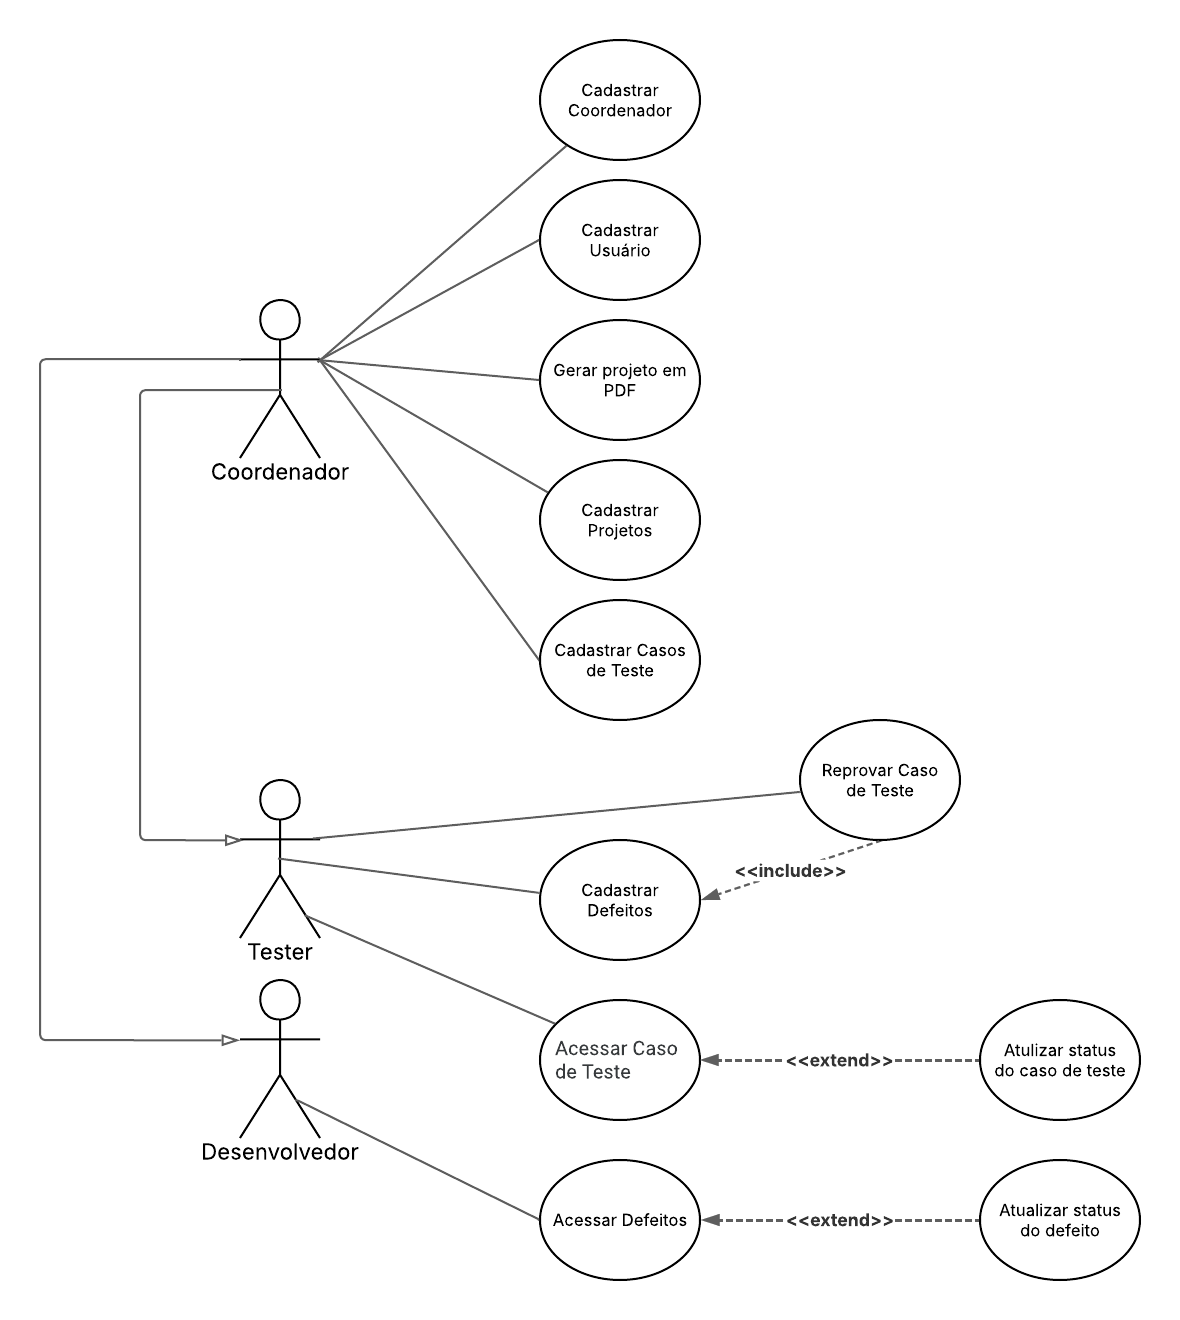
\includegraphics[width=0.88\textwidth, height=0.75\textheight, keepaspectratio]{./figuras/caso_uso_tcc.png} \\
    \vspace{0.2cm}
    {\raggedright \small Fonte: Elaborado pelo autor (2026).\par}
\end{figure}

\clearpage

\begin{quadro}[!htb]
\centering
\caption{Descrição dos Casos de Uso do sistema Test-Manager e sua relação com os Requisitos Funcionais.}
\label{tab:casos_uso}
\footnotesize
\begin{tabularx}{\textwidth}{|l|p{3.2cm}|X|l|}
\hline
\textbf{ID} & \textbf{Caso de Uso} & \textbf{Descrição do Comportamento} & \textbf{Requisitos} \\ \hline
UC01 & Cadastrar Coordenador & O usuário realiza seu próprio cadastro inicial no sistema com o perfil de coordenador. & RF01, RF02 \\ \hline
UC02 & Cadastrar Usuário & O Coordenador cadastra novos Testers e Desenvolvedores, vinculando-os ao ecossistema. & RF02, RF04 \\ \hline
UC03 & Gerar projeto em PDF & O Coordenador gera um relatório consolidado com as informações e métricas do projeto em formato PDF. & RF12, RF13 \\ \hline
UC04 & Cadastrar Projetos & O Coordenador gerencia o registro dos projetos de software da instituição e aloca a equipe. & RF03 \\ \hline
UC05 & Cadastrar Casos de Teste & O Coordenador cria ou importa em lote (.csv) os roteiros de teste e suas versões, associando-os aos projetos. & RF05, RF06, RF07, RF08 \\ \hline
UC06 & Acessar Caso de Teste & O Tester visualiza a lista e os detalhes dos casos de teste e versões atribuídos a ele. & RF05, RF08 \\ \hline
UC07 & Atualizar status do caso de teste & (Extensão de UC06) O Tester altera a situação da versão do teste após realizar sua avaliação prática. & RF09, RF13 \\ \hline
UC08 & Reprovar Caso de Teste & O Tester reprova um cenário de teste cuja execução falhou, iniciando o fluxo de relato da falha e geração de nova versão. & RF07, RF09, RF13 \\ \hline
UC09 & Cadastrar Defeitos & (Dependência de UC08) O Tester ou Coordenador registra os detalhes do bug encontrado, passos de reprodução, severidade e evidência visual. & RF10, RF13 \\ \hline
UC10 & Acessar Defeitos & O Desenvolvedor consulta os defeitos reportados nos projetos e atribuídos à sua responsabilidade. & RF10, RF11 \\ \hline
UC11 & Atualizar status do defeito & (Extensão de UC10) O Desenvolvedor atualiza o status de correção do defeito e gera histórico de auditoria das ações. & RF11, RF13 \\ \hline
\end{tabularx}
\fonte{Elaborado pelo autor (2026).}
\end{quadro}

\section{Modelagem Estrutural}

A modelagem estrutural abstrai a arquitetura interna do sistema, definindo como as informações são representadas no código-fonte por meio de classes e como essas entidades persistem no banco de dados relacional.

\subsection{Diagrama de Classes}

O Diagrama de Classes (Figura \ref{fig:diagrama_classes}) representa a estrutura orientada a objetos da aplicação, mapeando as classes de modelo (\textit{Models}) gerenciadas pelo Eloquent ORM do Laravel, seus atributos encapsulados (visibilidade privada `\texttt{-}'), métodos públicos de negócio e relacionamento (`\texttt{+}') e suas respectivas cardinalidades.

A classe \texttt{User} centraliza o controle de acesso por perfis (\texttt{coordenador}, \texttt{desenvolvedor} e \texttt{tester}) e possui um auto-relacionamento (\texttt{created\_by}) para rastrear qual coordenador cadastrou cada membro da equipe. A classe \texttt{Projeto} armazena o escopo, objetivos e critérios de entrada e saída, associando-se aos usuários de forma muitos-para-muitos por meio da classe associativa \texttt{ProjetoUser} (tabela pivô \texttt{projeto\_user}).

Cada \texttt{Projeto} agrega múltiplos registros de \texttt{CasoDeTeste}, que por sua vez compõem o histórico de auditoria (\texttt{Historico}), os ciclos de execução em \texttt{CasoVersao} (vinculados ao Tester responsável e ao avaliador) e os registros de \texttt{Defeito} (que conectam a falha encontrada na versão do teste ao usuário que a reportou e ao desenvolvedor designado em \texttt{responsavel\_dev}).

\begin{figure}[htbp]
    \centering
    \caption{Diagrama de Classes do sistema Test-Manager.}
    \label{fig:diagrama_classes}
    \vspace{0.15cm}
    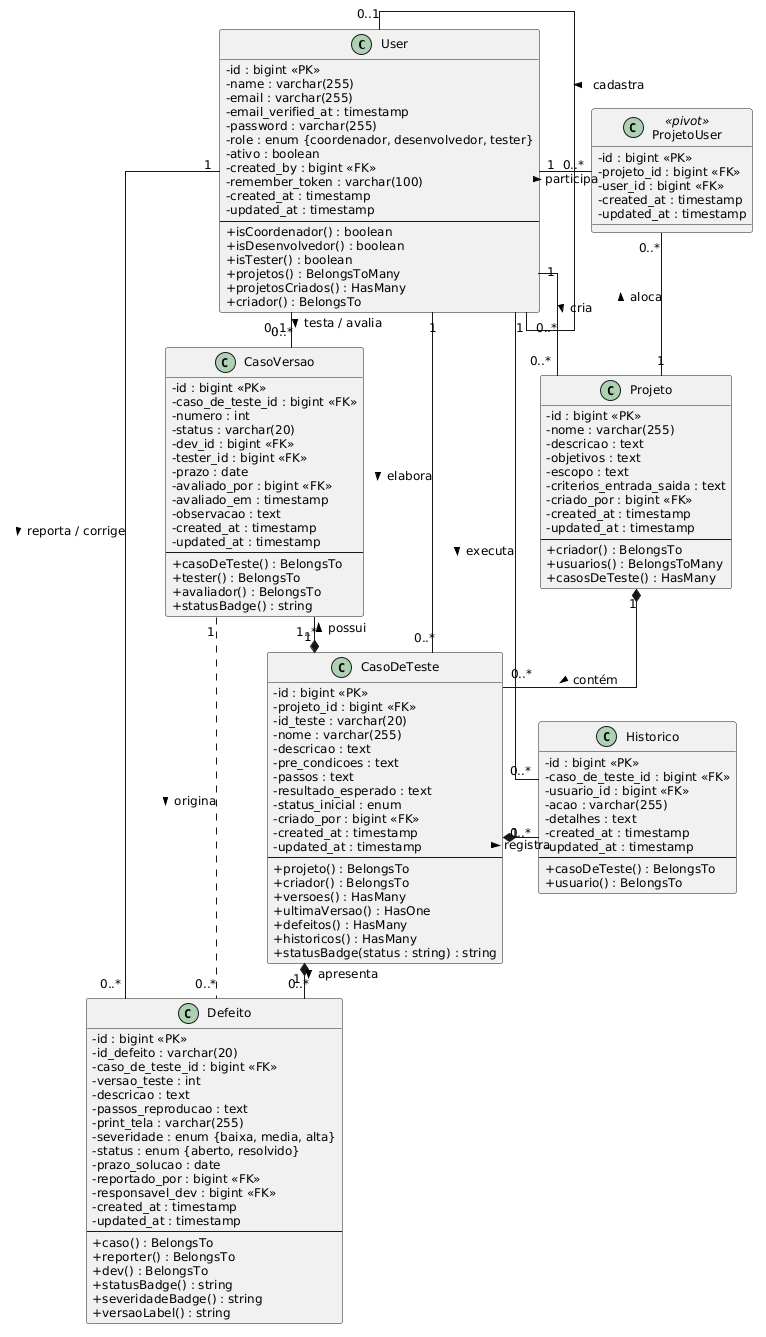
\includegraphics[width=1.0\textwidth, height=0.82\textheight, keepaspectratio]{./figuras/DiagramaDeClasse2.png} \\
    \vspace{0.15cm}
    {\raggedright \small Fonte: Elaborado pelo autor (2026).\par}
\end{figure}

\clearpage

\subsection{Modelo Lógico de Dados}

O armazenamento das informações orquestradas pelas classes do sistema exige uma infraestrutura relacional íntegra e normalizada. O Modelo Lógico do Banco de Dados, representado pelo Diagrama Entidade-Relacionamento (DER) na Figura \ref{fig:modelo_bd}, traduz a abstração orientada a objetos em tabelas físicas no SGBD MySQL, detalhando tipos de dados, chaves primárias (\texttt{PK}), chaves estrangeiras (\texttt{FK}) e restrições de integridade referencial.

No núcleo de domínio do banco de dados, a estrutura organiza-se em sete tabelas principais interligadas:
\begin{itemize}
    \item \textbf{\texttt{users}:} Armazena as credenciais de autenticação, o estado de ativação (\texttt{ativo}) e o papel de acesso (\texttt{role}) de cada usuário. Possui uma chave estrangeira auto-referenciada (\texttt{created\_by}) que aponta para o próprio \texttt{users(id)}, permitindo identificar o coordenador responsável pelo cadastro de cada membro;
    \item \textbf{\texttt{projetos} e \texttt{projeto\_user}:} A tabela \texttt{projetos} persiste os metadados de cada projeto de software (nome, descrição, objetivos, escopo e critérios de entrada/saída) e vincula seu autor via \texttt{criado\_por}. Como um projeto comporta múltiplos integrantes e um usuário pode atuar em diversos projetos, a tabela associativa \texttt{projeto\_user} resolve o relacionamento $N:N$ por meio das chaves estrangeiras \texttt{projeto\_id} e \texttt{user\_id};
    \item \textbf{\texttt{casos\_de\_teste}:} Registra a especificação base de cada roteiro de teste, incluindo o identificador amigável (\texttt{id\_teste}, como \texttt{CT-001}), pré-condições, passos de execução e resultado esperado, subordinando-se a um projeto (\texttt{projeto\_id}) e ao usuário autor (\texttt{criado\_por});
    \item \textbf{\texttt{caso\_versoes}:} Materializa o controle de versionamento dos testes (RF07). Em vez de sobrescrever o resultado de execuções anteriores, cada ciclo de avaliação gera uma linha vinculada a \texttt{caso\_de\_teste\_id}, contendo o número sequencial da versão (\texttt{numero}), o status (\texttt{pendente}, \texttt{aprovado} ou \texttt{reprovado}), o prazo limite, o avaliador designado (\texttt{tester\_id}) e os metadados de auditoria da execução (\texttt{avaliado\_por}, \texttt{avaliado\_em} e \texttt{observacao});
    \item \textbf{\texttt{defeitos}:} Centraliza os erros (\textit{bugs}) reportados durante a reprovação de um caso de teste. Além de vincular o caso de teste (\texttt{caso\_de\_teste\_id}) e o número da versão avaliada (\texttt{versao\_teste}), armazena o código identificador (\texttt{id\_defeito}, ex.: \texttt{DEF-001}), os passos para reprodução, o caminho da captura de tela (\texttt{print\_tela}), o nível de severidade (\texttt{baixa}, \texttt{media} ou \texttt{alta}), o status de resolução e as chaves estrangeiras que conectam o relator (\texttt{reportado\_por}) e o desenvolvedor encarregado da correção (\texttt{responsavel\_dev});
    \item \textbf{\texttt{historicos}:} Atua como uma trilha de auditoria imutável (RF13), registrando automaticamente cada evento relevante ocorrido no ciclo de vida de um caso de teste (\texttt{caso\_de\_teste\_id}), o autor da operação (\texttt{usuario\_id}), a descrição da ação (\texttt{acao}) e os detalhes da transição de estado (\texttt{detalhes}).
\end{itemize}

Complementarmente, o diagrama da Figura \ref{fig:modelo_bd} exibe à direita e nas extremidades as tabelas nativas de infraestrutura geradas pelas \textit{migrations} padrão do framework Laravel: \texttt{migrations} (controle de versão do esquema do banco), \texttt{sessions} e \texttt{password\_reset\_tokens} (gerenciamento de sessões ativas e recuperação de credenciais), \texttt{cache} e \texttt{cache\_locks} (otimização de consultas temporárias), bem como \texttt{jobs}, \texttt{job\_batches} e \texttt{failed\_jobs} (processamento de filas em segundo plano). O uso do mapeamento objeto-relacional (Eloquent ORM) atua como camada de abstração direta sobre o modelo físico representado na Figura \ref{fig:modelo_bd}, auxiliando na prevenção contra injeção de SQL e na manutenção da integridade dos dados.

\begin{figure}[!htb]
    \centering
    \caption{Modelo Lógico do Banco de Dados (DER) do Test-Manager.}
    \label{fig:modelo_bd}
    \vspace{0.2cm}
    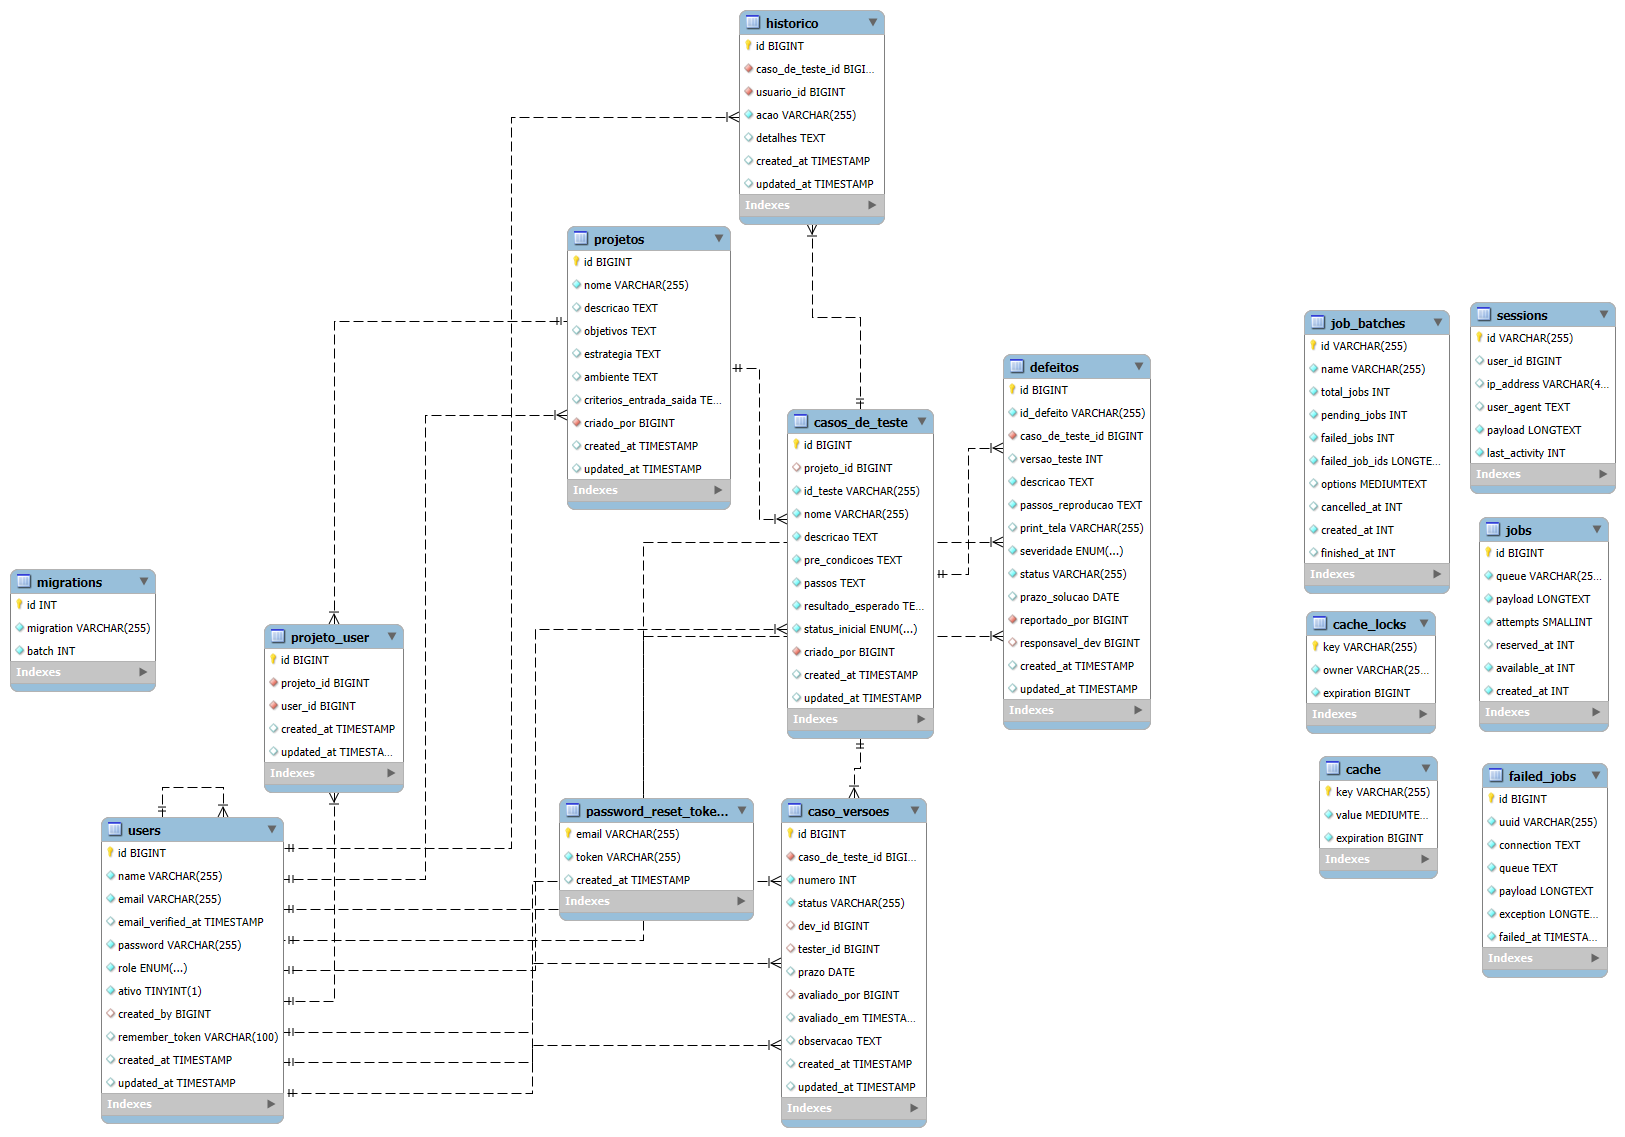
\includegraphics[width=0.98\textwidth, height=0.75\textheight, keepaspectratio]{./figuras/Modelobancodedados.png} \\
    \vspace{0.2cm}
    {\raggedright \small Fonte: Elaborado pelo autor (2026).\par}
\end{figure}
  \chapter{O Sistema Test-Manager}

Este capítulo apresenta o sistema Test-Manager implementado, detalhando a materialização prática da arquitetura planejada, o controle de acesso hierárquico por perfis e as interfaces gráficas que atendem aos requisitos funcionais e casos de uso especificados no Capítulo 4.

\section{Arquitetura da Solução e Controle de Acesso}

A solução adota uma arquitetura web monolítica estruturada sob o padrão \textit{Model-View-Controller} (MVC), implementada por meio do framework Laravel (PHP) em conjunto com o banco de dados relacional MySQL. No lado do servidor, os controladores (\textit{Controllers}) concentram as regras de negócio, a validação de formulários e a orquestração do versionamento de testes, enquanto a camada de persistência utiliza o mapeamento objeto-relacional Eloquent ORM para garantir a integridade referencial das transações. Na camada de apresentação (\textit{View}), o motor de templates Blade renderiza interfaces dinâmicas e responsivas estilizadas com o framework Bootstrap 5 (RNF01). Toda a infraestrutura executa de forma isolada em contêineres Docker, assegurando padronização entre os ambientes de desenvolvimento e implantação.

O controle de acesso e a segurança da plataforma (RF01, RF02 e RNF02) apoiam-se no mecanismo nativo de sessões autenticadas do Laravel, com senhas criptografadas via algoritmo BCrypt e proteção contra falsificação de requisições (\textit{CSRF Token}). A autorização operacional ocorre em duas frentes complementares:
\begin{itemize}
    \item \textbf{Restrição na camada de apresentação:} As diretivas condicionais do Blade ocultam botões de ação, menus e formulários não autorizados para o papel do usuário logado, adaptando a interface ao escopo de cada ator;
    \item \textbf{Validação estrita no servidor:} Os controladores e \textit{middlewares} verificam o atributo de perfil (\texttt{role}) e o vínculo do usuário com o projeto antes de processar qualquer requisição HTTP, bloqueando acessos diretos não autorizados via URL.
\end{itemize}

Dessa forma, o perfil \textbf{Coordenador} detém visibilidade administrativa sobre seus projetos, equipes, roteiros de teste e métricas; o \textbf{Tester} visualiza e executa exclusivamente os casos de teste e versões atribuídos à sua responsabilidade; e o \textbf{Desenvolvedor} acessa e atualiza estritamente os defeitos (\textit{bugs}) sob sua incumbência técnica.

\section{Interfaces e Fluxos Operacionais do Sistema}

O painel administrativo do Test-Manager materializa os módulos modelados no Capítulo 4. Para cada funcionalidade apresentada a seguir, descreve-se o fluxo operacional na perspectiva do usuário, relacionando os elementos visuais da tela às regras de negócio e aos requisitos funcionais correspondentes. O Quadro \ref{quad:modulos_sistema} sintetiza os módulos implementados e os perfis autorizados em cada etapa do fluxo de qualidade.

\begin{quadro}[!htb]
\centering
\caption{Módulos do sistema Test-Manager, funcionalidades e perfis de acesso.}
\label{quad:modulos_sistema}
\small
\begin{tabularx}{\textwidth}{|p{2.5cm}|X|p{3.4cm}|p{2.2cm}|}
\hline
\textbf{Módulo} & \textbf{Principais Funcionalidades} & \textbf{Perfis Autorizados} & \textbf{Requisitos} \\ \hline
Acesso & Autenticação de usuários, proteção de sessão e cadastro inicial de coordenador. & Todos os perfis & RF01, RF02 \\ \hline
Dashboard & Exibição de indicadores de testes (aprovados, reprovados, pendentes), defeitos por severidade e exportação de relatório em PDF. & Coordenador, Tester e Desenvolvedor & RF12 \\ \hline
Projetos e Equipe & Cadastro e gestão de projetos de software, cadastro de usuários e alocação de membros ($N:N$). & Coordenador & RF03, RF04 \\ \hline
Casos de Teste & Criação manual, importação em lote via arquivo \texttt{.csv}, versionamento automático e atribuição de Testers. & Coordenador (gestão) e Tester (consulta) & RF05, RF06, RF07, RF08 \\ \hline
Execução e Avaliação & Execução passo a passo do roteiro de teste, aprovação ou reprovação de versão com geração automática de nova versão. & Tester e Coordenador & RF07, RF09, RF13 \\ \hline
Defeitos (\textit{Bugs}) & Registro obrigatório de defeito na reprovação (com upload de \textit{print}), atribuição de desenvolvedor e atualização de status de correção. & Tester/Coordenador (registro) e Desenvolvedor (correção) & RF10, RF11, RF13 \\ \hline
\end{tabularx}
\fonte{Elaborado pelo autor (2026).}
\end{quadro}

\subsection{Acesso ao Sistema e Painel de Indicadores (Dashboard)}

\subsubsection{Login e Autenticação}

O acesso inicial ao Test-Manager materializa os requisitos RF01 e RF02 e o caso de uso UC01. Na tela de autenticação (Figura \ref{fig:tela_login}), o usuário informa seu endereço de e-mail institucional e senha. Caso as credenciais sejam válidas e o cadastro esteja ativo no banco de dados, o sistema inicia a sessão autenticada e redireciona o integrante diretamente ao painel principal configurado para o seu perfil de acesso.

\begin{figure}[H]
    \centering
    \caption{Tela de login e autenticação do Test-Manager.}
    \label{fig:tela_login}
    \vspace{0.2cm}
    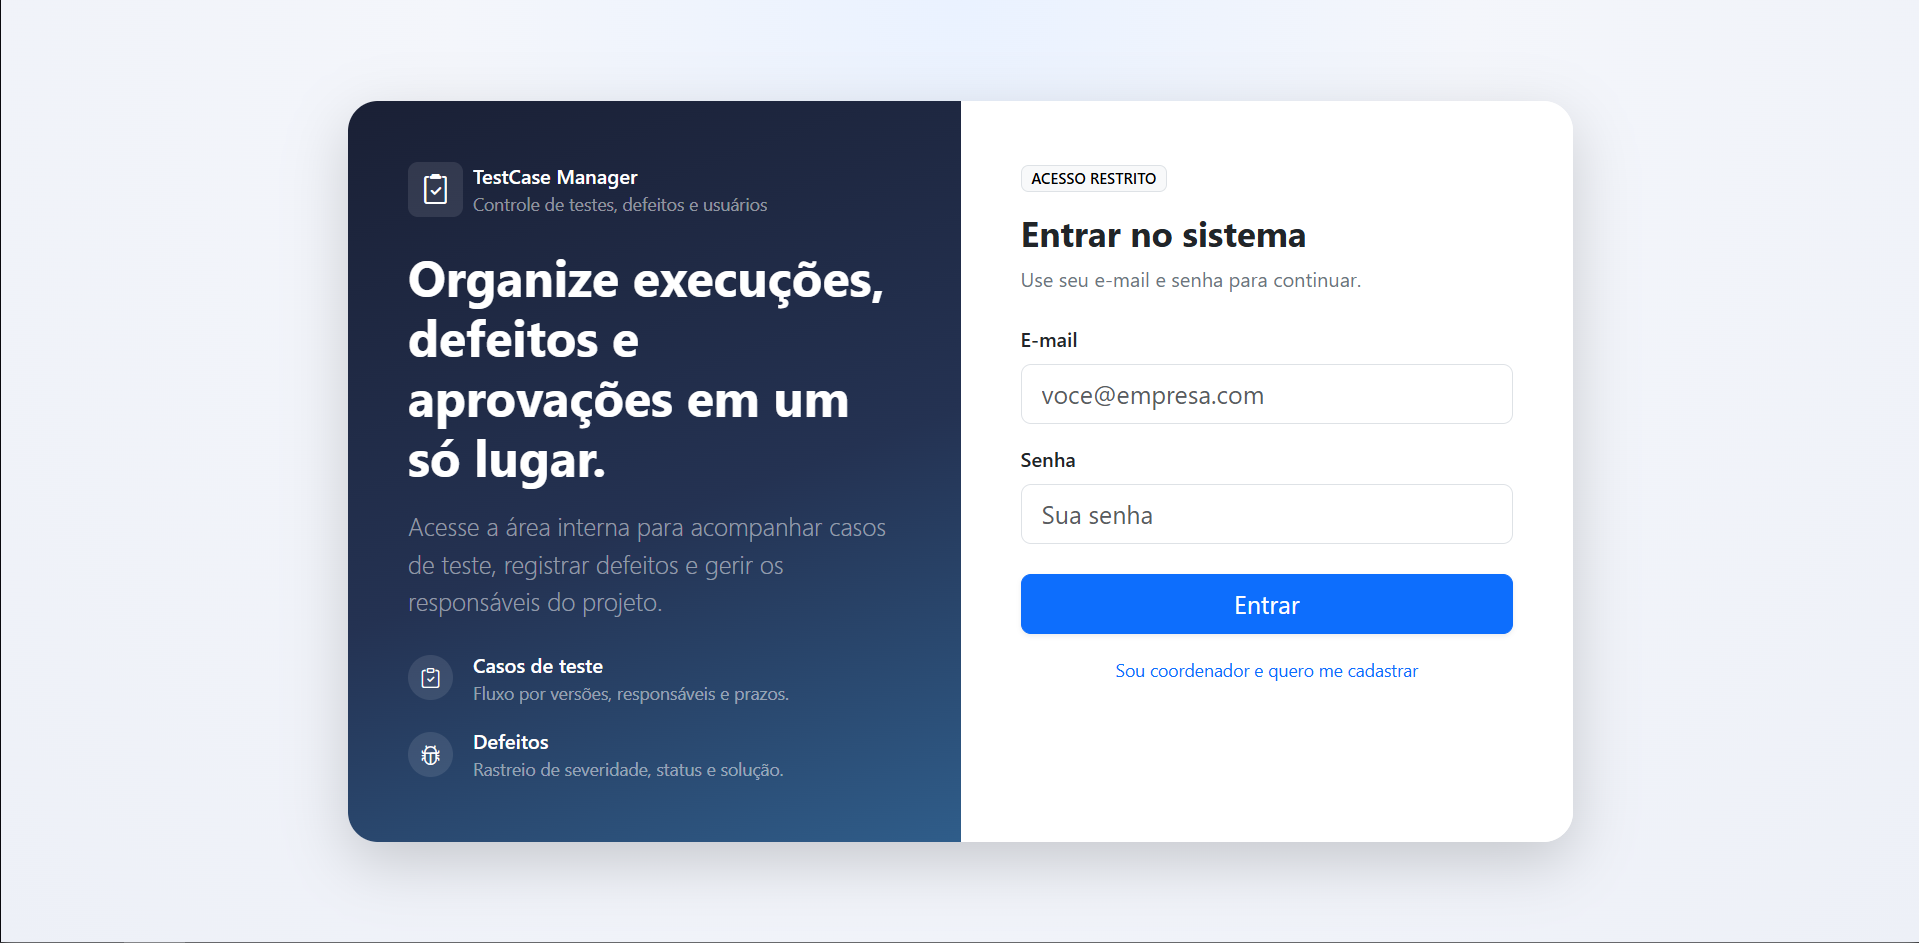
\includegraphics[width=0.85\textwidth, height=0.75\textheight, keepaspectratio]{./figuras/tela_login.png} \\
    \vspace{0.2cm}
    {\raggedright \small Fonte: Elaborado pelo autor (2026).\par}
\end{figure}

\subsubsection{Dashboard Gerencial e Relatórios}

Após a autenticação, o usuário visualiza o \textit{Dashboard} da plataforma (Figura \ref{fig:tela_dashboard}), que atende ao requisito RF12. Para o perfil Coordenador, o painel consolida em tempo real as métricas de qualidade dos projetos sob sua gestão, exibindo cartões totalizadores com o volume de projetos ativos, o total de casos de teste cadastrados, a proporção de versões aprovadas, pendentes e reprovadas, bem como a distribuição de defeitos abertos e resolvidos. Adicionalmente, o coordenador dispõe da funcionalidade de exportação consolidada em formato PDF (UC03), permitindo documentar o estado de estabilidade do software avaliado para fins acadêmicos e gerenciais.

\begin{figure}[H]
    \centering
    \caption{Painel de indicadores (Dashboard) do Test-Manager.}
    \label{fig:tela_dashboard}
    \vspace{0.2cm}
    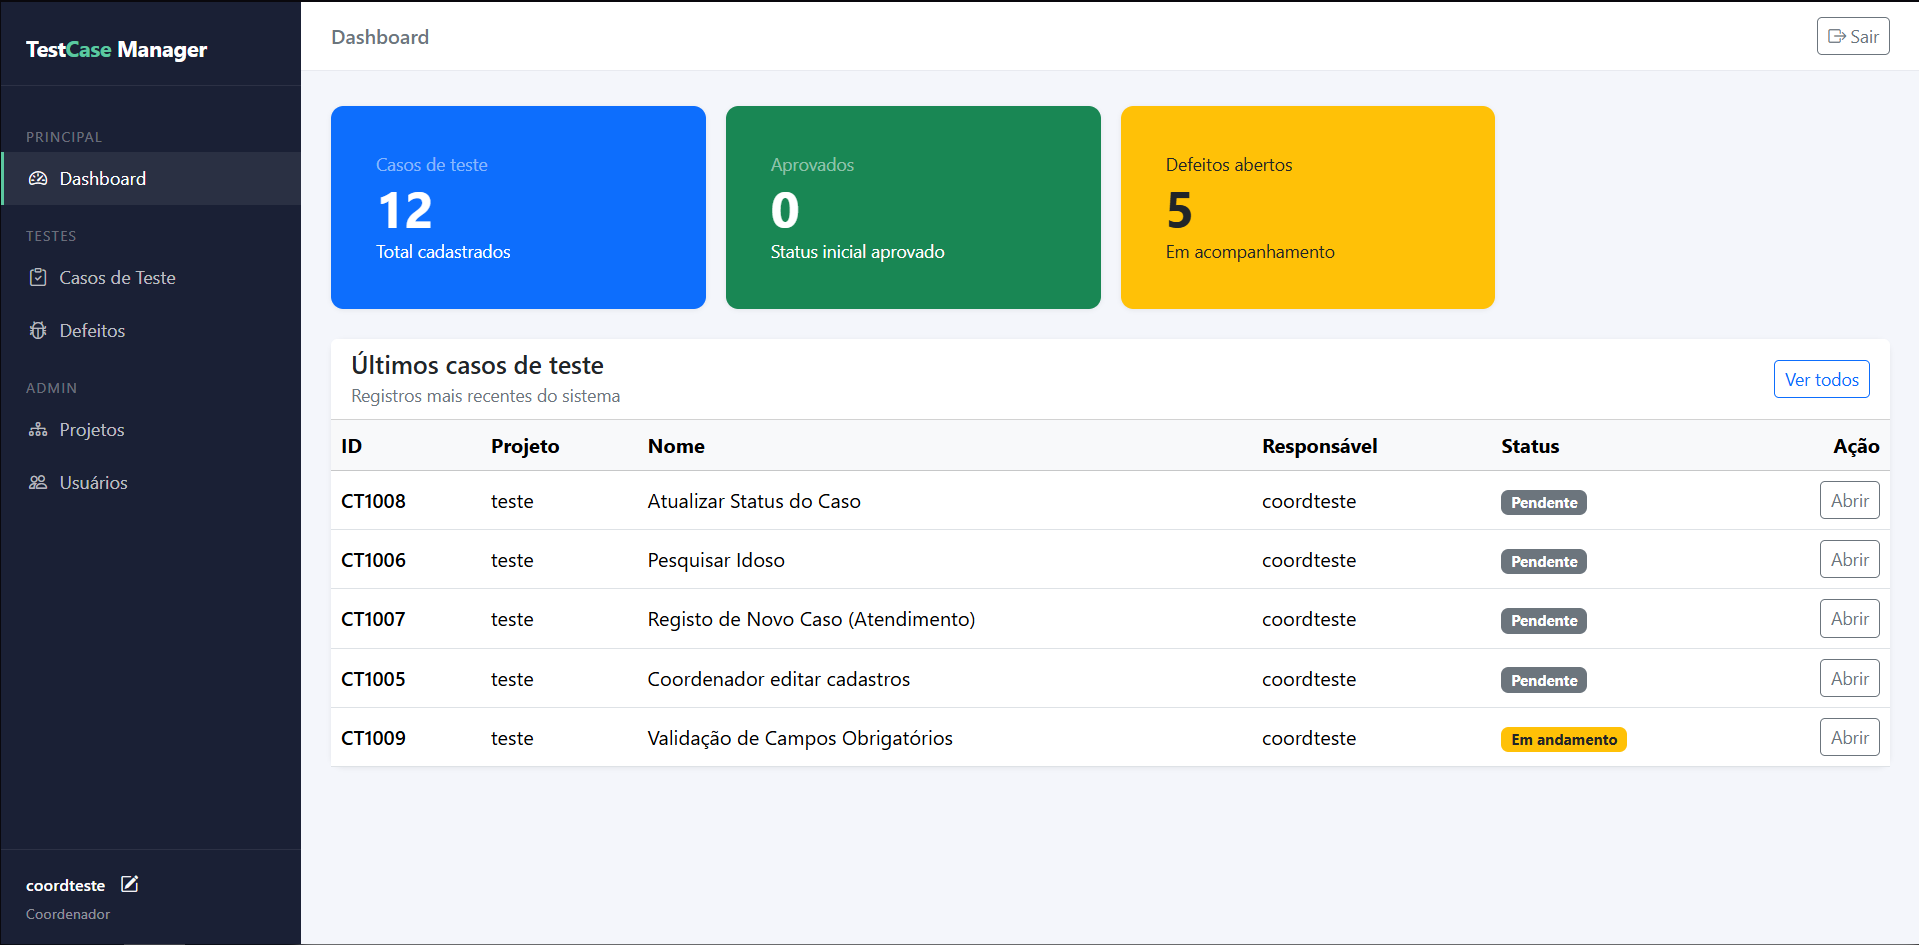
\includegraphics[width=0.92\textwidth, height=0.75\textheight, keepaspectratio]{./figuras/tela_dashboard.png} \\
    \vspace{0.2cm}
    {\raggedright \small Fonte: Elaborado pelo autor (2026).\par}
\end{figure}

\subsection{Gestão de Projetos, Equipes e Casos de Teste}

\subsubsection{Cadastro de Projetos e Alocação de Usuários}

Este módulo implementa os requisitos RF03 e RF04 (casos de uso UC02 e UC04). Na interface de gestão de projetos (Figura \ref{fig:tela_projetos}), o Coordenador registra os sistemas em desenvolvimento no campus, especificando nome, descrição, objetivos, escopo e critérios formais de entrada e saída. Na mesma estrutura, o coordenador cadastra novos usuários com os papéis de Tester ou Desenvolvedor e realiza a vinculação desses integrantes aos projetos correspondentes, garantindo que cada membro visualize apenas os artefatos das equipes em que está alocado.

\begin{figure}[H]
    \centering
    \caption{Tela de gestão de projetos e vinculação de equipe.}
    \label{fig:tela_projetos}
    \vspace{0.2cm}
    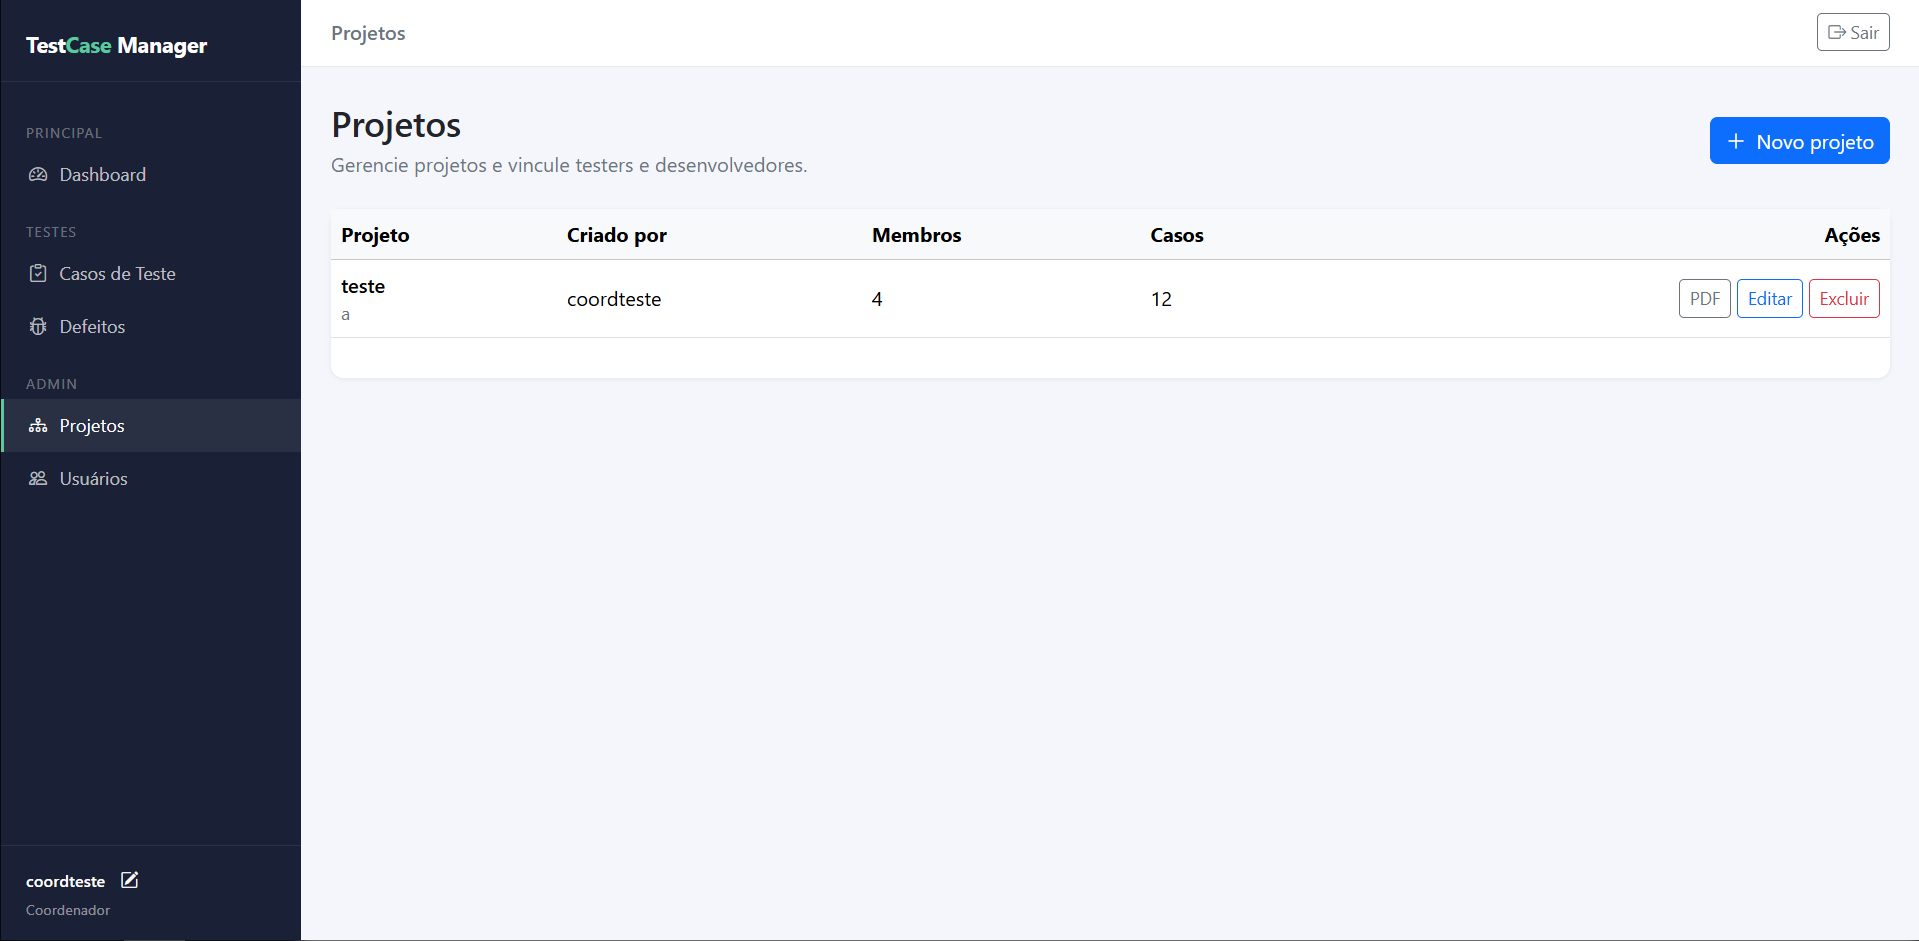
\includegraphics[width=0.92\textwidth, height=0.75\textheight, keepaspectratio]{./figuras/tela_projetos.png} \\
    \vspace{0.2cm}
    {\raggedright \small Fonte: Elaborado pelo autor (2026).\par}
\end{figure}

\subsubsection{Gestão de Casos de Teste e Importação em Lote}

A estruturação dos roteiros de validação contempla os requisitos RF05, RF06, RF07 e RF08 (UC05). Na tela de listagem e criação de casos de teste (Figura \ref{fig:tela_casos}), o Coordenador pode cadastrar cenários individualmente --- definindo título, descrição, pré-condições, passos sequenciais de execução, resultado esperado, prazo e Tester responsável --- ou utilizar a ferramenta de importação em lote mediante o envio de arquivos estruturados no formato \texttt{.csv}. Ao registrar um novo caso de teste, o sistema gera automaticamente um código identificador padronizado (como \texttt{CT-001}) e instancia sua versão inicial (\texttt{v1.0}) com status \textit{Pendente}, implementando paginação nas listagens (RNF03) para preservar a fluidez da navegação.

\begin{figure}[H]
    \centering
    \caption{Listagem e gerenciamento de casos de teste no painel.}
    \label{fig:tela_casos}
    \vspace{0.2cm}
    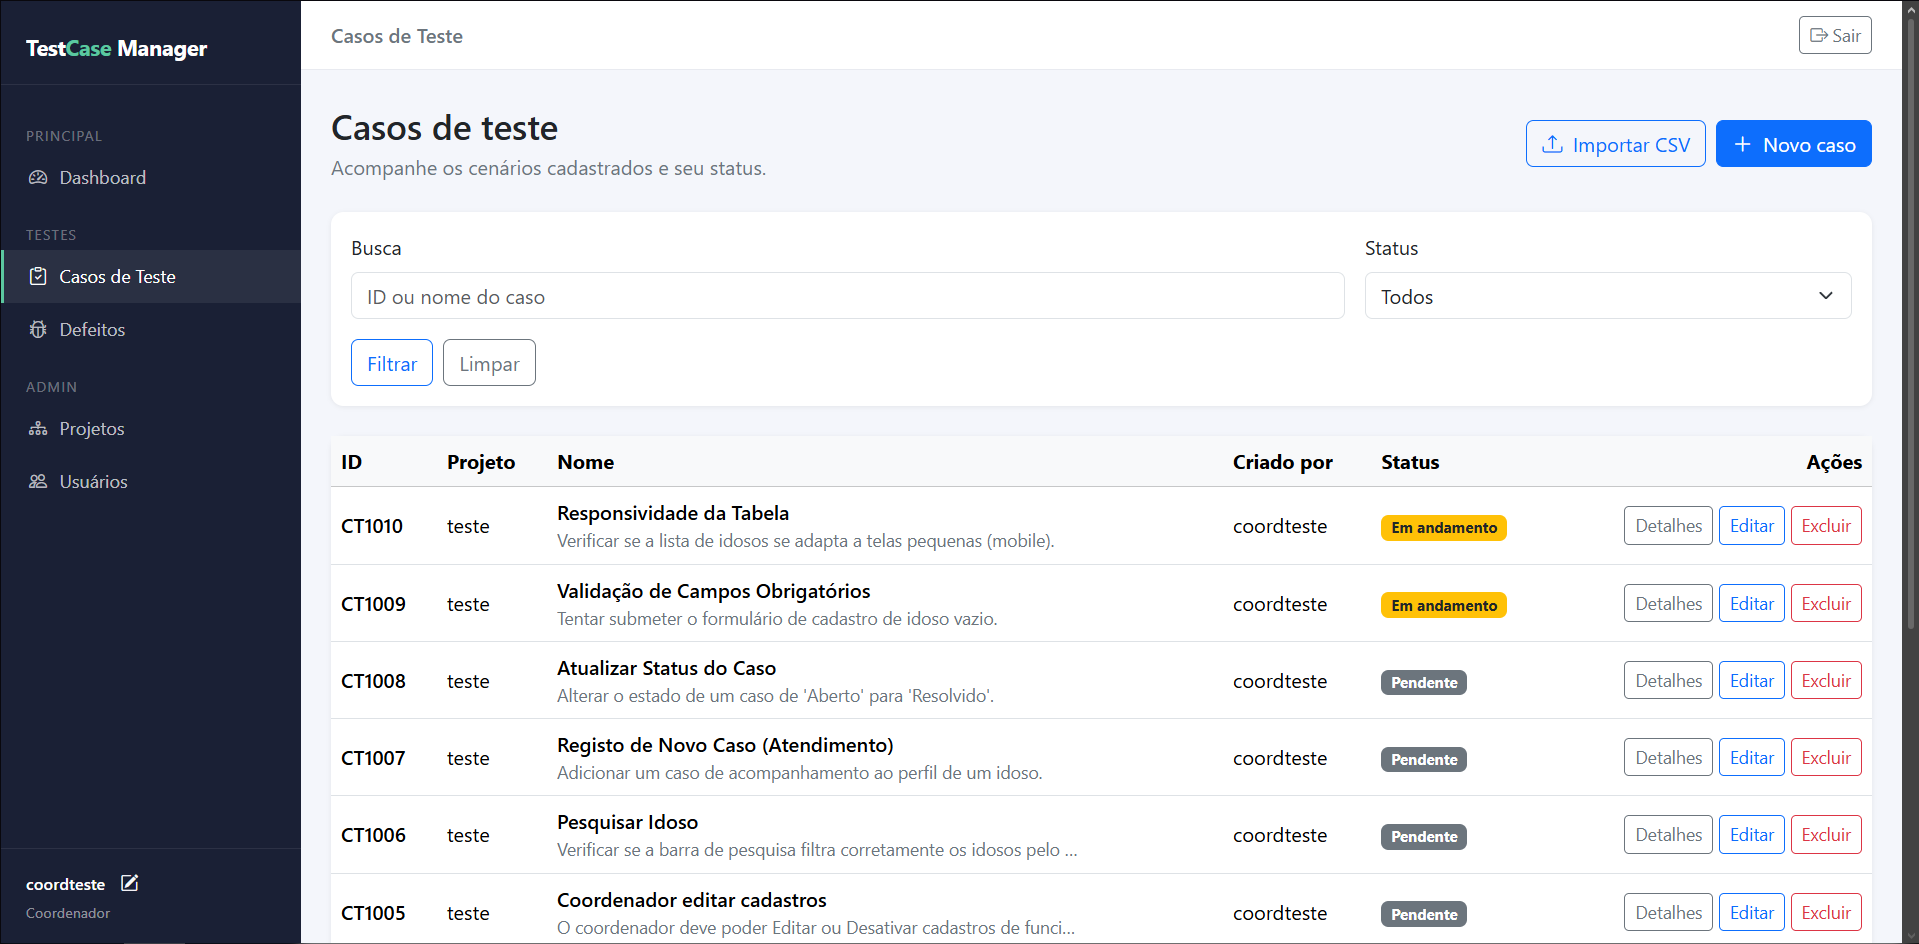
\includegraphics[width=0.92\textwidth, height=0.75\textheight, keepaspectratio]{./figuras/tela_casos.png} \\
    \vspace{0.2cm}
    {\raggedright \small Fonte: Elaborado pelo autor (2026).\par}
\end{figure}

\subsection{Execução de Testes, Rastreamento de Defeitos e Auditoria}

\subsubsection{Execução de Casos de Teste e Versionamento Automático}

O módulo de avaliação operacionaliza os requisitos RF07, RF09 e RF13 (casos de uso UC06, UC07 e UC08). Ao acessar os detalhes de um caso de teste atribuído ao seu perfil (Figura \ref{fig:tela_execucao_caso}), o Tester inspeciona as pré-condições, os passos de reprodução e o resultado esperado da versão ativa. Caso o software avaliado se comporte conforme especificado, o Tester aprova a versão, encerrando o ciclo de validação daquele cenário. Por outro lado, caso seja constatada uma falha durante a execução, o acionamento da reprovação retém a avaliação em sessão e direciona o usuário obrigatoriamente ao formulário de registro de defeito. Concluído o relato da falha, o sistema consolida a versão atual como \textit{Reprovada}, cria automaticamente a versão subsequente (\texttt{v2.0}, \texttt{v3.0}) com status \textit{Pendente} para reteste futuro e grava o evento na linha do tempo de auditoria (\texttt{Historico}) exibida na própria tela.

\begin{figure}[H]
    \centering
    \caption{Tela de detalhes do caso de teste, avaliação de versões e histórico de auditoria.}
    \label{fig:tela_execucao_caso}
    \vspace{0.2cm}
    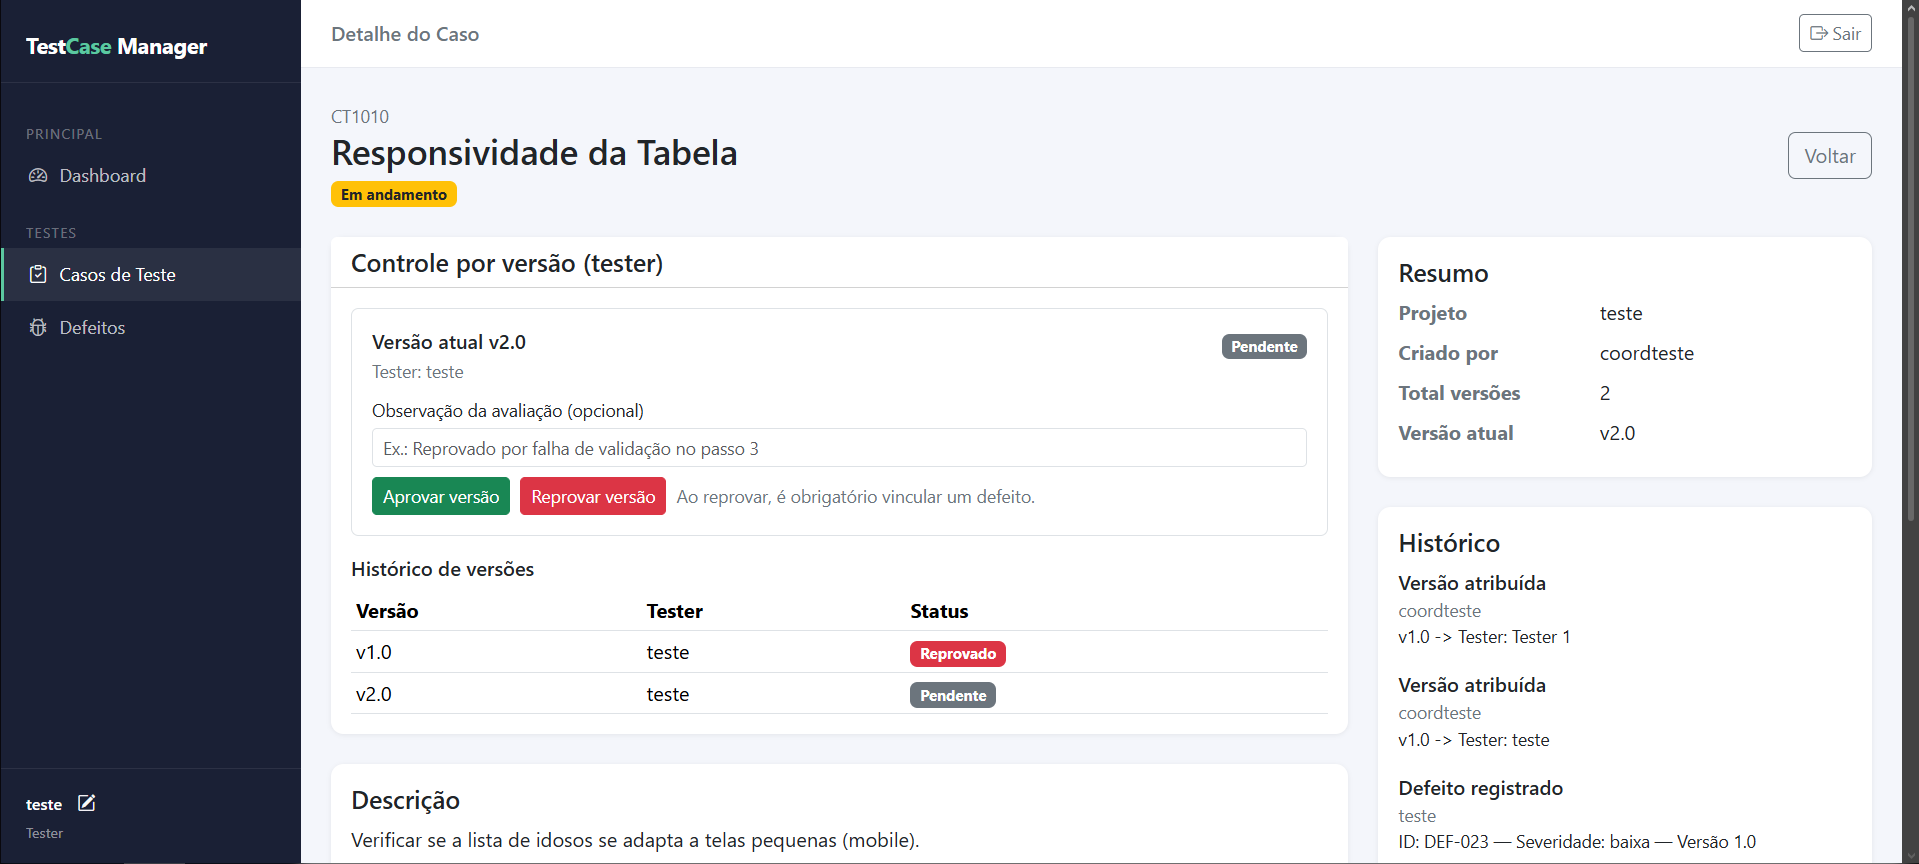
\includegraphics[width=0.92\textwidth, height=0.75\textheight, keepaspectratio]{./figuras/tela_execucao_caso.png} \\
    \vspace{0.2cm}
    {\raggedright \small Fonte: Elaborado pelo autor (2026).\par}
\end{figure}

\subsubsection{Registro e Ciclo de Vida de Defeitos (Bugs)}

O gerenciamento de falhas atende aos requisitos RF10, RF11 e RF13 (casos de uso UC09, UC10 e UC11). Na tela de registro e acompanhamento de defeitos (Figura \ref{fig:tela_defeitos}), o relator documenta a anomalia informando a versão do teste afetada, a descrição detalhada do problema, os passos exatos para reprodução, o grau de severidade (\textit{Baixa}, \textit{Média} ou \textit{Alta}) e anexa a captura de tela (\textit{print}) que evidencia o erro visualmente. O Coordenador designa o Desenvolvedor responsável e estipula o prazo de solução. Na visão do Desenvolvedor, o painel lista todos os defeitos sob sua responsabilidade, permitindo consultar os passos e evidências anexadas e atualizar o status do registro para \textit{Resolvido} assim que a correção do código-fonte é finalizada, notificando a rastreabilidade no histórico do caso de teste correspondente.

\begin{figure}[H]
    \centering
    \caption{Módulo de registro e acompanhamento do ciclo de vida de defeitos.}
    \label{fig:tela_defeitos}
    \vspace{0.2cm}
    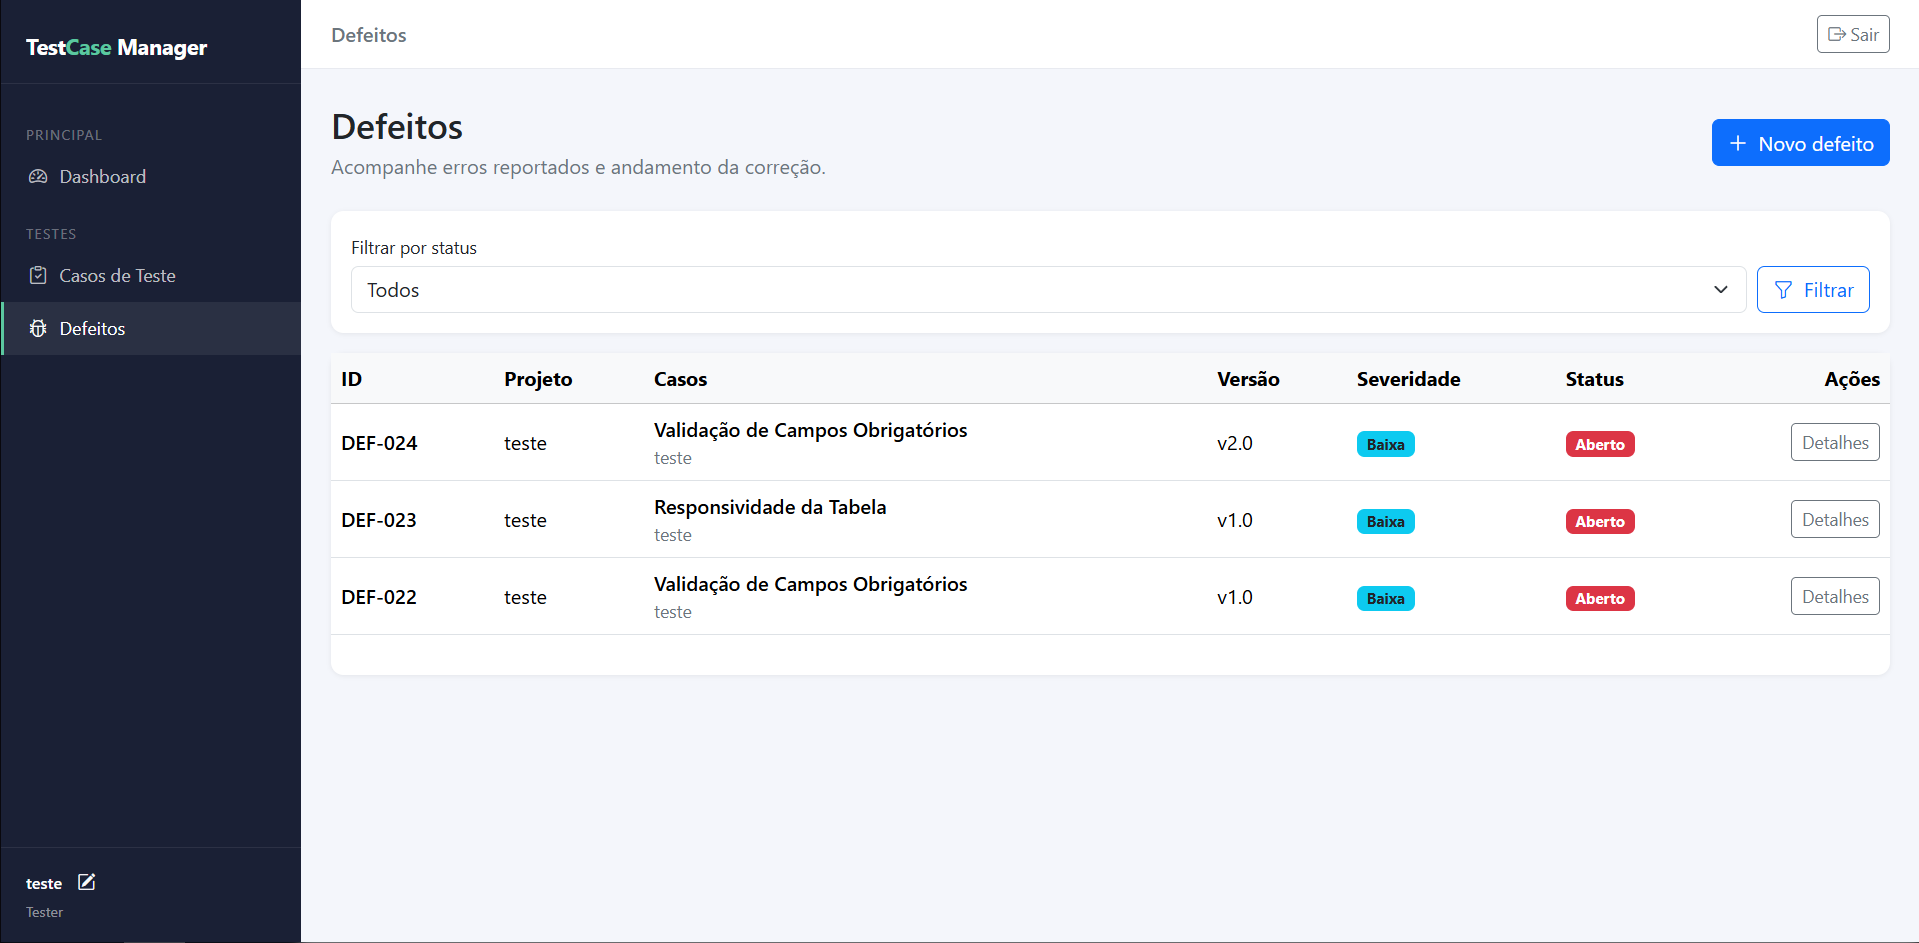
\includegraphics[width=0.92\textwidth, height=0.75\textheight, keepaspectratio]{./figuras/tela_defeitos.png} \\
    \vspace{0.2cm}
    {\raggedright \small Fonte: Elaborado pelo autor (2026).\par}
\end{figure}
  \chapter{Validação do Sistema (Resultados e Discussão)}

Este capítulo apresenta os resultados da validação do sistema Test-Manager junto aos usuários que atuaram nos papéis de Coordenador, Tester e Desenvolvedor em projetos de software do IFES Campus Alegre. O delineamento metodológico geral da avaliação foi descrito no Capítulo 3; nesta seção detalham-se o instrumento ramificado por perfil, o protocolo de coleta, a tabulação estatística das respostas e a discussão dos achados em relação aos objetivos do trabalho.

\section{Instrumentos de Avaliação}

A validação foi estruturada em dois níveis complementares: (i) verificação técnica funcional por lista de checagem (\textit{checklist}) dos fluxos operacionais e restrições de acesso por perfil; e (ii) avaliação perceptiva dos usuários por meio de questionário estruturado fundamentado no Modelo de Aceitação de Tecnologia (\textit{Technology Acceptance Model} --- TAM) \cite{davis1989, venkatesh2000} e em preceitos de engenharia de usabilidade \cite{nielsen1994}.

\subsection{Verificação Técnica}

Antes da aplicação do questionário, foram exercitados manualmente os fluxos principais do sistema em ambiente conteinerizado: cadastro de projetos e alocação de equipes pelo Coordenador, importação de roteiros de teste em lote via arquivo \texttt{.csv}, atribuição e avaliação de versões pelo Tester, exigência de cadastro de defeito com upload de captura de tela (\textit{print}) no fluxo de reprovação, atualização de status de correção pelo Desenvolvedor e geração de logs de auditoria e relatórios em PDF. Confirmou-se que as regras de negócio modeladas no Capítulo 4 refletem-se integralmente no comportamento da aplicação, sem falhas de permissão entre perfis.

\subsection{Questionário de Avaliação (Modelo TAM)}

O questionário foi elaborado na plataforma Google Forms e organizado em blocos lógicos. O primeiro bloco coletou o perfil de acesso principal utilizado pelo participante e apresentou oito afirmações gerais (Q1 a Q8), respondidas por todos os integrantes, abrangendo os construtos de \textbf{Facilidade de Uso Percebida} (Q1 a Q3), \textbf{Utilidade Percebida} (Q4 a Q6) e \textbf{Intenção Comportamental de Uso} (Q7 e Q8).

Na sequência, o formulário utilizou ramificação condicional para avaliar as funcionalidades exclusivas de cada ator: o perfil \textbf{Coordenador} respondeu aos itens Q9 a Q11; o perfil \textbf{Tester} avaliou os itens Q12 a Q14; e o perfil \textbf{Desenvolvedor} respondeu aos itens Q15 a Q17. Todas as afirmações fechadas foram mensuradas em escala Likert de cinco pontos, variando de 1 (\textit{Discordo Totalmente}) a 5 (\textit{Concordo Totalmente}). Ao final, duas questões abertas (Q18 e Q19) coletaram percepções sobre dificuldades encontradas e sugestões de evolução futura. O Quadro \ref{quad:itens_questionario} detalha a estrutura completa do instrumento aplicado.

\begin{quadro}[!htb]
\centering
\caption{Itens do formulário de avaliação do sistema Test-Manager.}
\label{quad:itens_questionario}
\footnotesize
\begin{tabularx}{\textwidth}{|p{1.1cm}|p{3.3cm}|X|}
\hline
\textbf{Cód.} & \textbf{Dimensão / Escopo} & \textbf{Afirmação / Questão} \\ \hline
Perfil & Identificação & Qual é o seu perfil de acesso principal no Test-Manager? (Coordenador, Tester ou Desenvolvedor). \\ \hline
Q1 & Facilidade de Uso (Geral) & Aprender a utilizar o Test-Manager foi um processo fácil e rápido para mim. \\ \hline
Q2 & Facilidade de Uso (Geral) & A interface do sistema é clara, intuitiva e fácil de navegar. \\ \hline
Q3 & Facilidade de Uso (Geral) & É fácil encontrar as informações ou funcionalidades que preciso dentro do sistema. \\ \hline
Q4 & Utilidade Percebida (Geral) & O uso do Test-Manager torna o processo mais rápido em comparação ao método anterior (planilhas/Google Docs). \\ \hline
Q5 & Utilidade Percebida (Geral) & O sistema ajuda a manter o histórico de testes e falhas de forma mais segura e rastreável. \\ \hline
Q6 & Utilidade Percebida (Geral) & Em geral, acredito que o Test-Manager melhora a minha produtividade no projeto. \\ \hline
Q7 & Intenção de Uso (Geral) & Pretendo continuar utilizando o Test-Manager nas atividades de QA dos próximos projetos. \\ \hline
Q8 & Intenção de Uso (Geral) & Eu recomendaria este sistema para outras equipes de desenvolvimento do IFES. \\ \hline
Q9 & Específico: Coordenador & O processo de criar projetos e vincular Desenvolvedores e Testers é simples e direto. \\ \hline
Q10 & Específico: Coordenador & O sistema me oferece uma boa visão geral sobre o andamento da qualidade dos projetos. \\ \hline
Q11 & Específico: Coordenador & A importação em lote de casos de teste via arquivo CSV agiliza a alimentação inicial do sistema. \\ \hline
Q12 & Específico: Tester & A tela de listagem de Casos de Teste permite entender rapidamente os passos e o resultado esperado. \\ \hline
Q13 & Específico: Tester & O processo de aprovar ou reprovar uma versão de teste é ágil e requer poucos cliques. \\ \hline
Q14 & Específico: Tester & A obrigatoriedade de cadastrar um defeito (\textit{bug}) ao reprovar um teste ajuda a garantir a documentação da falha. \\ \hline
Q15 & Específico: Desenvolvedor & É fácil visualizar e filtrar os defeitos (\textit{bugs}) que foram atribuídos ao meu projeto. \\ \hline
Q16 & Específico: Desenvolvedor & As informações fornecidas na tela de Detalhes do Defeito são claras e suficientes para eu corrigir o erro. \\ \hline
Q17 & Específico: Desenvolvedor & Atualizar o ciclo de vida do defeito facilita a comunicação com a equipe sem usar ferramentas externas. \\ \hline
Q18 & Aberta (Dificuldades) & Qual foi a maior dificuldade ou confusão que você encontrou ao utilizar o sistema? \\ \hline
Q19 & Aberta (Sugestões) & Quais funcionalidades você sugere que sejam adicionadas, alteradas ou removidas no futuro? \\ \hline
\end{tabularx}
\fonte{Elaborado pelo autor (2026).}
\end{quadro}

\section{Procedimento de Coleta}

O procedimento adotado na condução da avaliação empírica seguiu cinco etapas:
\begin{enumerate}
    \item Disponibilização do Test-Manager aos participantes atuantes em projetos de software no IFES Campus Alegre, com orientação inicial conforme o perfil de acesso;
    \item Período de uso orientado do sistema contemplando os fluxos de criação de projetos, importação e cadastro de casos de teste, execução e avaliação de versões, relato obrigatório de defeitos na reprovação e resolução de \textit{bugs};
    \item Divulgação do link do formulário eletrônico aos usuários que operaram a plataforma;
    \item Coleta anônima das respostas por meio do Google Forms entre outubro e novembro de 2026;
    \item Tabulação quantitativa das respostas em escala Likert (médias aritméticas e desvios-padrão amostrais) e análise qualitativa das respostas discursivas.
\end{enumerate}

Não houve identificação nominal dos participantes; o perfil declarado serviu exclusivamente para direcionar o bloco de questões específicas e contextualizar a análise dos resultados.

\section{Resultados}

A coleta obteve 5 respostas válidas ($n = 5$) após o uso orientado do Test-Manager. Quanto ao perfil de acesso principal declarado, a amostra contemplou todos os atores modelados no sistema, distribuindo-se em: Coordenador (1), Tester (2) e Desenvolvedor (2).

A Tabela \ref{tab:resultados_likert} consolida o número de respondentes ($n$), as médias e os desvios-padrão (DP) obtidos em cada afirmação na escala de 1 a 5. De forma complementar, a Figura \ref{fig:grafico_pizza_concordancia} apresenta em gráficos de setores (pizza) a proporção percentual das notas atribuídas no bloco geral (Q1 a Q8) e nos módulos específicos por perfil (Q9 a Q17), enquanto a Figura \ref{fig:grafico_pizza_dimensoes_tam} detalha a distribuição percentual de concordância estratificada pelas três dimensões do Modelo TAM.

\begin{table}[H]
\centering
\caption{Resultados do questionário de avaliação do Test-Manager (Escala Likert 1--5).}
\label{tab:resultados_likert}
\small
\begin{tabularx}{\textwidth}{|l|X|c|c|c|}
\hline
\textbf{Item} & \textbf{Aspecto Avaliado} & \textbf{$n$} & \textbf{Média} & \textbf{DP} \\ \hline
\multicolumn{5}{|l|}{\textbf{Dimensões Gerais do Modelo TAM (Todos os Perfis)}} \\ \hline
Q1 & Facilidade e rapidez no aprendizado do sistema & 5 & 4,20 & 0,45 \\ \hline
Q2 & Clareza, intuitividade e navegabilidade da interface & 5 & 4,40 & 0,89 \\ \hline
Q3 & Facilidade para localizar informações e funcionalidades & 5 & 4,20 & 0,84 \\ \hline
Q4 & Agilidade do processo frente a planilhas/Google Docs & 5 & 4,40 & 0,89 \\ \hline
Q5 & Segurança e rastreabilidade do histórico de testes e falhas & 5 & 4,80 & 0,45 \\ \hline
Q6 & Melhoria da produtividade nas atividades do projeto & 5 & 4,60 & 0,55 \\ \hline
Q7 & Intenção de uso contínuo nos próximos projetos & 5 & 4,60 & 0,55 \\ \hline
Q8 & Recomendação do sistema para outras equipes do IFES & 5 & 4,20 & 1,30 \\ \hline
\multicolumn{5}{|l|}{\textbf{Módulos Específicos por Perfil de Acesso}} \\ \hline
Q9 & Simplicidade ao criar projetos e vincular equipe (Coordenador) & 1 & 4,00 & - \\ \hline
Q10 & Visão geral sobre o andamento da qualidade (Coordenador) & 1 & 5,00 & - \\ \hline
Q11 & Agilidade na importação em lote via arquivo CSV (Coordenador) & 1 & 5,00 & - \\ \hline
Q12 & Clareza dos passos e resultado esperado na listagem (Tester) & 2 & 4,50 & 0,71 \\ \hline
Q13 & Agilidade ao aprovar ou reprovar versões de teste (Tester) & 2 & 5,00 & 0,00 \\ \hline
Q14 & Documentação garantida pelo defeito obrigatório na reprovação (Tester) & 2 & 5,00 & 0,00 \\ \hline
Q15 & Facilidade ao visualizar e filtrar defeitos atribuídos (Desenvolvedor) & 2 & 4,50 & 0,71 \\ \hline
Q16 & Suficiência das informações nos detalhes do defeito (Desenvolvedor) & 2 & 5,00 & 0,00 \\ \hline
Q17 & Comunicação facilitada pela atualização do ciclo de vida (Desenvolvedor) & 2 & 5,00 & 0,00 \\ \hline
\multicolumn{2}{|l|}{\textbf{Média Geral dos Itens Comuns (Q1--Q8)}} & \textbf{40 obs.} & \textbf{4,43} & \textbf{0,75} \\ \hline
\multicolumn{2}{|l|}{\textbf{Média Geral dos Módulos Específicos (Q9--Q17)}} & \textbf{15 obs.} & \textbf{4,80} & \textbf{0,41} \\ \hline
\multicolumn{2}{|l|}{\textbf{Média Global Consolidada (Q1--Q17)}} & \textbf{55 obs.} & \textbf{4,53} & \textbf{0,69} \\ \hline
\end{tabularx}
\fonte{Elaborado pelo autor (2026), com base na aplicação do questionário.}
\end{table}

\begin{figure}[H]
    \centering
    \caption{Proporção percentual de concordância na Escala Likert: (a) Dimensões Gerais (Q1 a Q8) e (b) Funcionalidades Específicas por Perfil (Q9 a Q17).}
    \label{fig:grafico_pizza_concordancia}
    \vspace{0.2cm}
    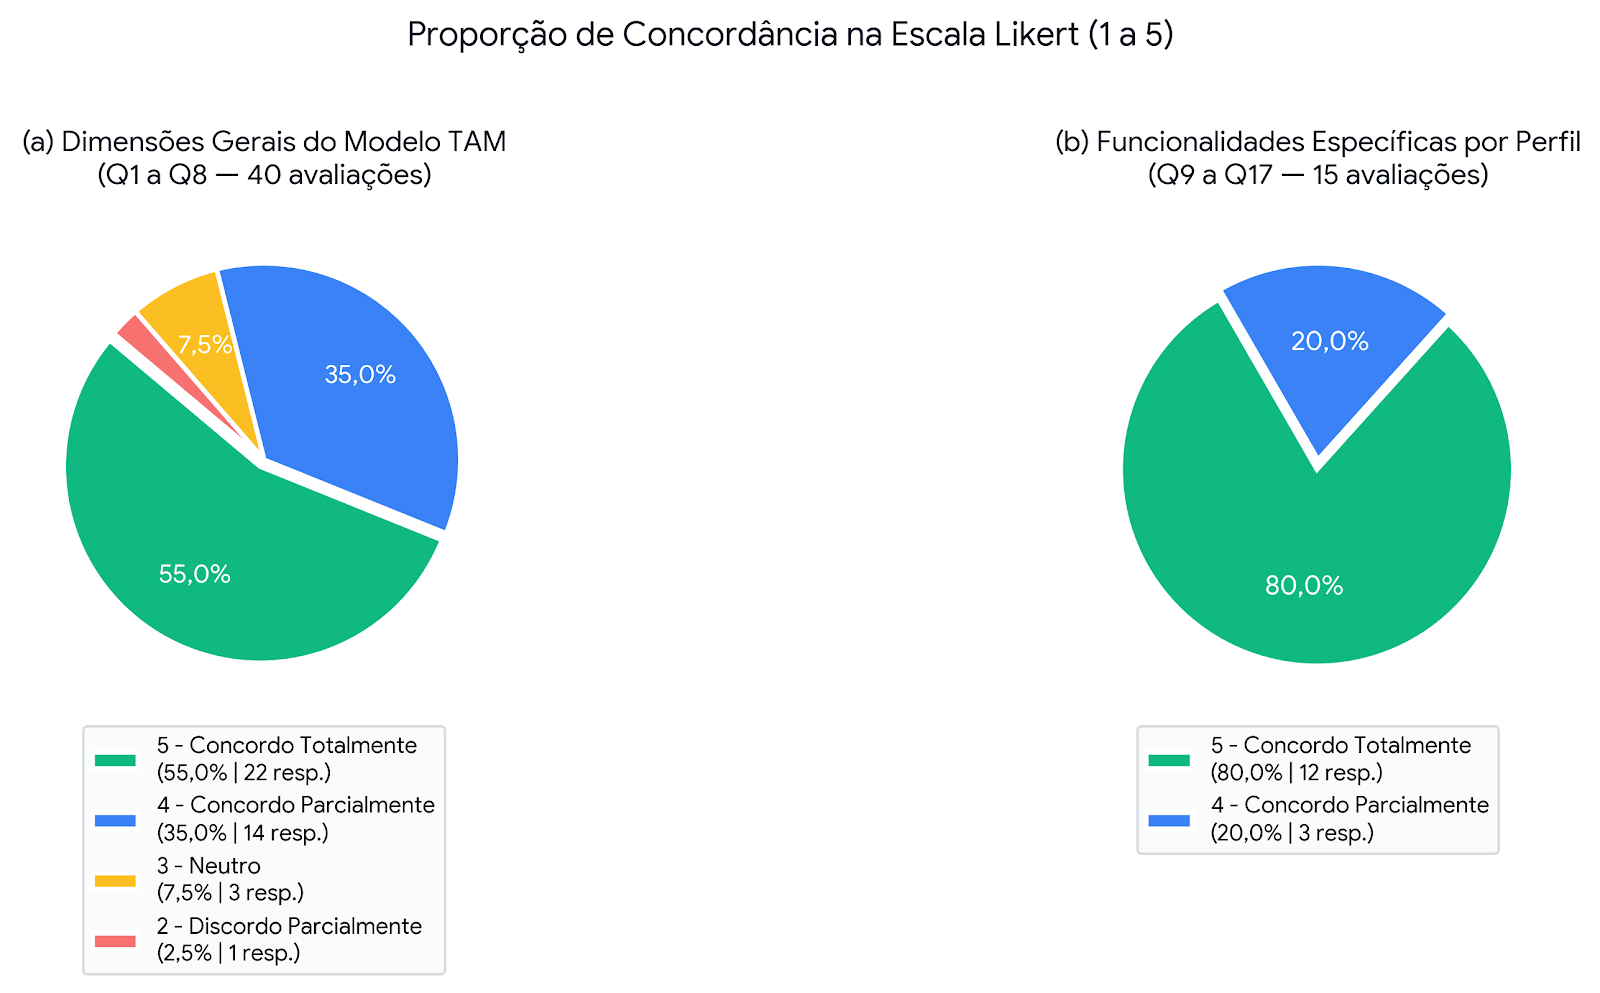
\includegraphics[width=0.95\textwidth, keepaspectratio]{./figuras/grafico_pizza_concordancia.png} \\
    \vspace{0.2cm}
    {\raggedright \small Fonte: Elaborado pelo autor (2026).\par}
\end{figure}

\begin{figure}[H]
    \centering
    \caption{Distribuição percentual das respostas por dimensão do Modelo TAM: (a) Facilidade de Uso, (b) Utilidade Percebida e (c) Intenção de Uso.}
    \label{fig:grafico_pizza_dimensoes_tam}
    \vspace{0.2cm}
    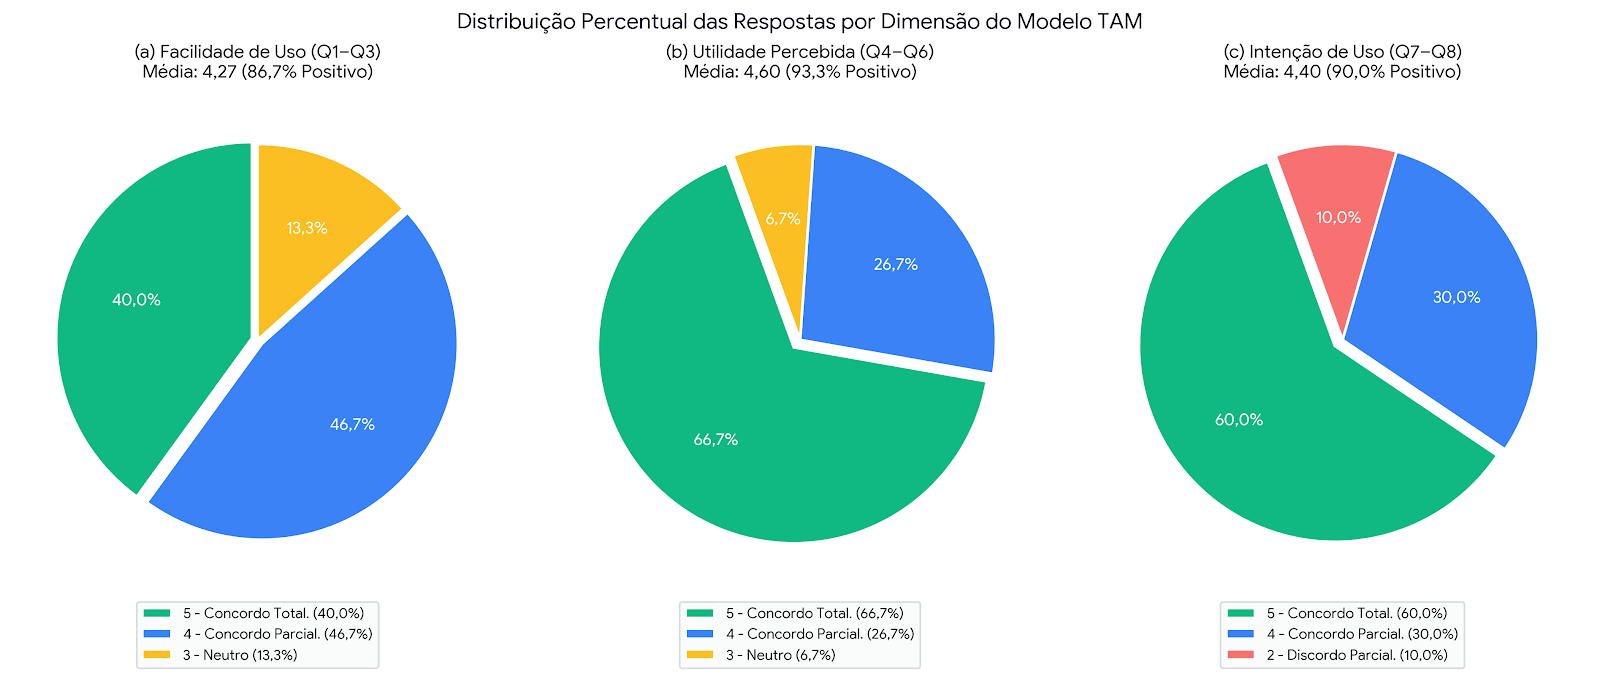
\includegraphics[width=0.98\textwidth, keepaspectratio]{./figuras/grafico_pizza_dimensoes_tam.png} \\
    \vspace{0.2cm}
    {\raggedright \small Fonte: Elaborado pelo autor (2026).\par}
\end{figure}

\subsection{Respostas Abertas: Dificuldades e Sugestões (Q18 e Q19)}

Nas questões discursivas destinadas ao levantamento de dificuldades operacionais (Q18) e sugestões de aprimoramento futuro (Q19), quatro participantes registraram observações sobre dificuldades e três indicaram propostas de evolução:
\begin{itemize}
    \item \textbf{Perfil Coordenador:} Relatou que sua expectativa inicial era de que a plataforma também abrangesse o gerenciamento prévio de requisitos do software, sugerindo para trabalhos futuros a inclusão de um módulo de cadastro de requisitos formalmente atrelado aos casos de teste, além do refinamento contínuo nas nomenclaturas de status de testes e níveis de prioridade de defeitos;
    \item \textbf{Perfil Tester:} Um avaliador apontou como limitação pontual o fato de o formulário de relato de defeito permitir o envio de apenas uma captura de tela (\textit{print}) por registro; o segundo avaliador mencionou dificuldade visual para localizar de imediato os botões de edição e exclusão logo após cadastrar um caso de teste, sugerindo destacá-los na interface de listagem;
    \item \textbf{Perfil Desenvolvedor:} Ambos os respondentes indicaram não ter encontrado nenhuma dificuldade ou confusão ao operar o sistema (``Nenhuma''), e um deles corroborou a sugestão de permitir o anexo de múltiplos arquivos ou imagens no registro de defeitos para enriquecer a evidência do erro.
\end{itemize}

\section{Discussão}

Conforme demonstrado na Tabela \ref{tab:resultados_likert} e ilustrado nos gráficos de setores das Figuras \ref{fig:grafico_pizza_concordancia} e \ref{fig:grafico_pizza_dimensoes_tam}, a avaliação empírica evidenciou ampla aceitação do sistema Test-Manager após o uso prático. Na Figura \ref{fig:grafico_pizza_concordancia}(a), observa-se que, das 40 avaliações individuais realizadas nas questões gerais (Q1 a Q8), expressivos \textbf{90,0\%} concentraram-se na faixa positiva de concordância --- sendo \textbf{55,0\%} (22 respostas) em \textit{Concordo Totalmente} (nota 5) e \textbf{35,0\%} (14 respostas) em \textit{Concordo Parcialmente} (nota 4) ---, frente a apenas 7,5\% (3 respostas) de posicionamento neutro e 2,5\% (1 resposta) de discordância parcial, resultando na média geral comum de 4,43 ($\text{DP} = 0,75$).

Analisando a Figura \ref{fig:grafico_pizza_dimensoes_tam}, que decompõe o resultado geral nas três dimensões teóricas do Modelo TAM \cite{davis1989, venkatesh2000}, verifica-se o predomínio das fatias de aprovação (verde e azul) em todos os construtos:
\begin{itemize}
    \item Na \textbf{Utilidade Percebida} (Figura \ref{fig:grafico_pizza_dimensoes_tam}b, referente aos itens Q4 a Q6), o índice de concordância positiva atingiu \textbf{93,3\%}, com dois terços das respostas (\textbf{66,7\%}) na nota máxima (\textit{Concordo Totalmente}) e média agregada de 4,60 ($\text{DP} = 0,63$). O destaque recaiu sobre o item Q5 (manutenção do histórico de testes e falhas de forma segura e rastreável, média 4,80), confirmando que a centralização em banco relacional supera a perda de histórico típica de planilhas e documentos soltos em nuvem \cite{medeiros2022, kokubum2025};
    \item Na \textbf{Facilidade de Uso Percebida} (Figura \ref{fig:grafico_pizza_dimensoes_tam}a, itens Q1 a Q3), \textbf{86,7\%} das respostas situaram-se entre \textit{Concordo Totalmente} (40,0\%) e \textit{Concordo Parcialmente} (46,7\%), com 13,3\% de neutralidade e nenhuma discordância (média de 4,27; $\text{DP} = 0,70$), validando a intuitividade da interface construída com Bootstrap 5;
    \item Na \textbf{Intenção Comportamental de Uso} (Figura \ref{fig:grafico_pizza_dimensoes_tam}c, itens Q7 e Q8), \textbf{90,0\%} das avaliações foram positivas (60,0\% em \textit{Concordo Totalmente} e 30,0\% em \textit{Concordo Parcialmente}, média 4,40). Os 10,0\% correspondentes a uma única resposta \textit{Discordo Parcialmente} (nota 2 em Q8) referem-se à cautela apontada pelo perfil Coordenador na questão aberta (Q18/Q19), que sugeriu incorporar um módulo prévio de Engenharia de Requisitos antes de expandir a recomendação da ferramenta para outras equipes.
\end{itemize}

Por fim, o gráfico da Figura \ref{fig:grafico_pizza_concordancia}(b) evidencia o desempenho superior do sistema na execução das rotinas específicas de cada papel (\textbf{Módulos Específicos por Perfil}, Q9 a Q17): \textbf{100,0\%} das 15 avaliações foram positivas, sendo \textbf{80,0\%} (12 respostas) de aprovação máxima (\textit{Concordo Totalmente}, nota 5) e \textbf{20,0\%} (3 respostas) de concordância parcial (nota 4), elevando a média específica para \textbf{4,80} ($\text{DP} = 0,41$). Seis dos nove indicadores específicos obtiveram nota máxima unânime (5,00): visão geral da qualidade (Q10) e importação em lote via CSV (Q11) no perfil Coordenador; agilidade ao aprovar/reprovar versões (Q13) e obrigatoriedade de abertura de defeito na reprovação (Q14) no perfil Tester; e clareza nos detalhes do defeito (Q16) e facilidade de comunicação pelo ciclo de vida (Q17) no perfil Desenvolvedor.

As sugestões registradas nas questões abertas --- suporte a múltiplos anexos de imagem por defeito, maior destaque visual aos botões de edição/exclusão para o perfil Tester e criação de um módulo de rastreabilidade de requisitos --- oferecem um direcionamento claro para a evolução contínua da plataforma, detalhado no Capítulo 7.
  \chapter{Conclusão}

Este capítulo apresenta uma síntese do trabalho desenvolvido, relaciona os resultados alcançados aos objetivos geral e específicos estabelecidos na introdução, discute as limitações identificadas ao longo da pesquisa e elenca diretrizes para trabalhos futuros.

\section{Considerações Finais}

O presente trabalho apresentou o projeto, o desenvolvimento e a validação do sistema web \textbf{Test-Manager}, concebido para centralizar o gerenciamento de casos de teste e o rastreamento de defeitos (\textit{bugs}) nos projetos de software do Instituto Federal do Espírito Santo (IFES) Campus Alegre. A proposta originou-se da necessidade prática de substituir controles descentralizados e informais --- baseados em documentos de texto e planilhas compartilhadas em nuvem ---, os quais ocasionavam perda recorrente de histórico de execução, desorganização de roteiros e dificuldade de acompanhamento gerencial pelos professores orientadores.

Guiado pela abordagem metodológica de Apresentação de Produto \cite{wazlawick2019} e por um processo de desenvolvimento iterativo e incremental, o estudo percorreu as etapas de elicitação de requisitos, modelagem arquitetural em UML, implementação sob o padrão Model-View-Controller (MVC) com o framework Laravel e banco de dados relacional MySQL em ambiente Docker, culminando na validação empírica com usuários reais. O artefato resultante consolidou em uma plataforma única o cadastro de projetos, a alocação de equipes, o controle automático de versões de testes (\texttt{v1.0}, \texttt{v2.0}), a obrigatoriedade de relato de defeitos em cenários reprovados e a trilha de auditoria imutável.

A validação conduzida após o uso orientado confirmou a elevada aceitação da plataforma pelas equipes, registrando forte reconhecimento quanto à utilidade prática, à segurança na preservação do histórico e à clareza na comunicação entre Coordenadores, Testers e Desenvolvedores. Conclui-se, portanto, que o Test-Manager cumpriu seu propósito tecnológico e acadêmico, oferecendo ao campus uma infraestrutura padronizada e auditável para o exercício prático da Garantia da Qualidade de Software (QA).

\section{Síntese do Atendimento aos Objetivos}

Em relação ao \textbf{objetivo geral} --- desenvolver um sistema web centralizado em PHP/Laravel e MySQL para otimizar o controle de qualidade, a preservação do histórico e a governança dos projetos de software do IFES Campus Alegre ---, verifica-se que a meta foi integralmente cumprida, com a solução projetada, codificada, conteinerizada e validada empiricamente.

Os \textbf{objetivos específicos} definidos na Seção 1.3.2 foram alcançados da seguinte forma:
\begin{itemize}
    \item \textbf{Mapeamento e especificação de requisitos:} Foram elicitados e documentados 13 Requisitos Funcionais (RF01 a RF13) e 3 Requisitos Não Funcionais essenciais (RNF01 a RNF03) a partir da análise das demandas reais das equipes de desenvolvimento e coordenação do campus (Capítulo 4);
    \item \textbf{Modelagem arquitetural e relacional:} A estrutura lógica e comportamental do sistema foi integralmente especificada por meio do Diagrama de Casos de Uso (11 casos de uso rastreáveis), do Diagrama de Classes orientado aos modelos do Eloquent ORM e do Modelo Lógico de Dados (DER) no SGBD MySQL (Seções 4.4 e 4.5);
    \item \textbf{Implementação do sistema Test-Manager:} A aplicação web foi construída sob o padrão MVC, contemplando o controle de acesso por perfis (Coordenador, Tester e Desenvolvedor), gestão de projetos, importação em lote de testes via CSV, versionamento automático de execuções, registro de defeitos com captura de tela, linha do tempo de auditoria e exportação de relatórios em PDF (Capítulo 5);
    \item \textbf{Execução de testes funcionais e validação com usuários:} Além da verificação técnica de todos os fluxos operacionais, aplicou-se o questionário baseado no Modelo TAM ($n = 5$, cobrindo todos os perfis), obtendo-se média geral de \textbf{4,43} nos itens comuns (Q1--Q8), média de \textbf{4,80} nas funcionalidades específicas de cada perfil (Q9--Q17) e média global consolidada de \textbf{4,53} na escala de 1 a 5 (Capítulo 6).
\end{itemize}

\section{Limitações}

A despeito dos resultados positivos alcançados, cumpre reconhecer algumas limitações inerentes ao escopo e ao recorte metodológico deste estudo:
\begin{itemize}
    \item \textbf{Delimitação de escopo ao ciclo de testes e defeitos:} O sistema foi projetado especificamente para gerenciar casos de teste, versões de execução e rastreamento de \textit{bugs}, não contemplando um módulo prévio de elicitação e gerenciamento de Requisitos Funcionais e Não Funcionais dos projetos avaliados;
    \item \textbf{Anexo único de evidência por defeito:} Na versão atual, o formulário de registro de defeito permite a anexação de apenas um arquivo de imagem (\textit{print} da tela) por ocorrência reportada;
    \item \textbf{Tamanho da amostra e estudo de caso único:} A validação empírica foi conduzida no contexto institucional específico do IFES Campus Alegre com uma amostra de cinco participantes ($n = 5$), o que, embora represente todos os papéis do sistema, impõe cautela na generalização estatística para outros cenários organizacionais;
    \item \textbf{Execução manual dos roteiros de teste:} A plataforma gerencia o planejamento, a versão e o veredito dos casos de teste executados por avaliadores humanos, não realizando a execução automatizada de scripts de teste de código (como testes unitários ou \textit{end-to-end}).
\end{itemize}

\section{Trabalhos Futuros}

Com base nas limitações identificadas e nas sugestões colhidas junto aos usuários durante a etapa de validação (Q18 e Q19), destacam-se as seguintes oportunidades de evolução contínua para o Test-Manager:
\begin{itemize}
    \item \textbf{Módulo de Engenharia de Requisitos e Matriz de Rastreabilidade:} Implementar o cadastro de requisitos de software dentro de cada projeto, permitindo vincular diretamente quais casos de teste validam determinado requisito e quais defeitos o impactam, atendendo à sugestão do perfil Coordenador;
    \item \textbf{Suporte a múltiplos anexos e vídeos nos defeitos:} Expandir a camada de armazenamento para permitir o envio de múltiplas capturas de tela, arquivos de log ou gravações curtas de tela em um único relato de \textit{bug}, conforme sugerido pelos perfis Tester e Desenvolvedor;
    \item \textbf{Refinamento de usabilidade e personalização de fluxos:} Aprimorar a visibilidade dos atalhos de edição e exclusão nas listagens de casos de teste e permitir a parametrização customizada de nomenclaturas de status e níveis de prioridade de defeitos por projeto;
    \item \textbf{Sistema de notificações ativas:} Integrar o envio automático de alertas por e-mail ou \textit{webhooks} (Discord, Telegram ou Slack) sempre que um teste for atribuído a um Tester, um defeito for designado a um Desenvolvedor ou uma correção for concluída;
    \item \textbf{Integração com repositórios Git e pipelines CI/CD:} Desenvolver integração via API com o GitHub e GitLab para vincular o fechamento de defeitos diretamente a \textit{commits} ou \textit{Pull Requests} e importar resultados de suítes de testes automatizados (PHPUnit, Jest ou Cypress).
\end{itemize}

\section{Considerações Finais do Autor}

A elaboração deste Trabalho de Conclusão de Curso proporcionou a consolidação prática das competências construídas ao longo da graduação em Tecnologia em Análise e Desenvolvimento de Sistemas no IFES Campus Alegre, integrando conhecimentos de Engenharia de Requisitos, Modelagem Orientada a Objetos, Banco de Dados, Arquitetura MVC com Laravel, Conteinerização com Docker e Qualidade de Software.

Mais do que a codificação de um artefato tecnológico, a vivência de diagnosticar uma necessidade real do ambiente acadêmico, projetar uma solução sob medida e submetê-la ao crivo de coordenadores, testadores e desenvolvedores evidenciou como a Engenharia de Software pode transformar processos informais em fluxos organizados, transparentes e colaborativos. Espera-se que o Test-Manager continue apoiando os projetos de ensino, pesquisa e extensão do campus e sirva como base evolutiva para as futuras gerações de estudantes da instituição.
    
  % --------------------------------------------------- %
  % ELEMENTOS POS-TEXTUAIS                              %
  % --------------------------------------------------- %
  \postextual
  
  % Referencias Bibliográficas
  \bibliographystyle{abntex2-alf} % Autor-Data
  \bibliography{bibliografia}
    
  % Apêndices
  %\begin{apendicesenv}
  %  \chapter{{\normalfont Explicação}}
\label{apendice: a}

É um elemento opcional. É um documento elaborado pelo próprio autor com o objetivo de completar sua argumentação, sem que haja prejuízo para a unidade do trabalho (ASSOCIAÇÃO BRASILEIRA DE NORMAS TÉCNICAS, 2011b. Deve ser precedido da palavra APÊNDICE (ex:APÊNDICE A, APÊNDICE B), identificado por letras maiúsculas consecutivas, travessão e pelo respectivo título. 
  %\end{apendicesenv}

  % Anexos
  \begin{anexosenv}
    \partanexos
    \chapter{Relatório do Projeto e Execução de Casos de Teste Gerado pelo Sistema Test-Manager}
    \label{anexo:relatorio_pdf}

    A seguir, apresenta-se o documento em formato PDF exportado pelo perfil Coordenador diretamente na listagem de projetos do sistema Test-Manager (Caso de Uso UC03), contendo os metadados do projeto, a equipe vinculada, a linha do tempo dos casos de teste e o resumo das versões executadas.

    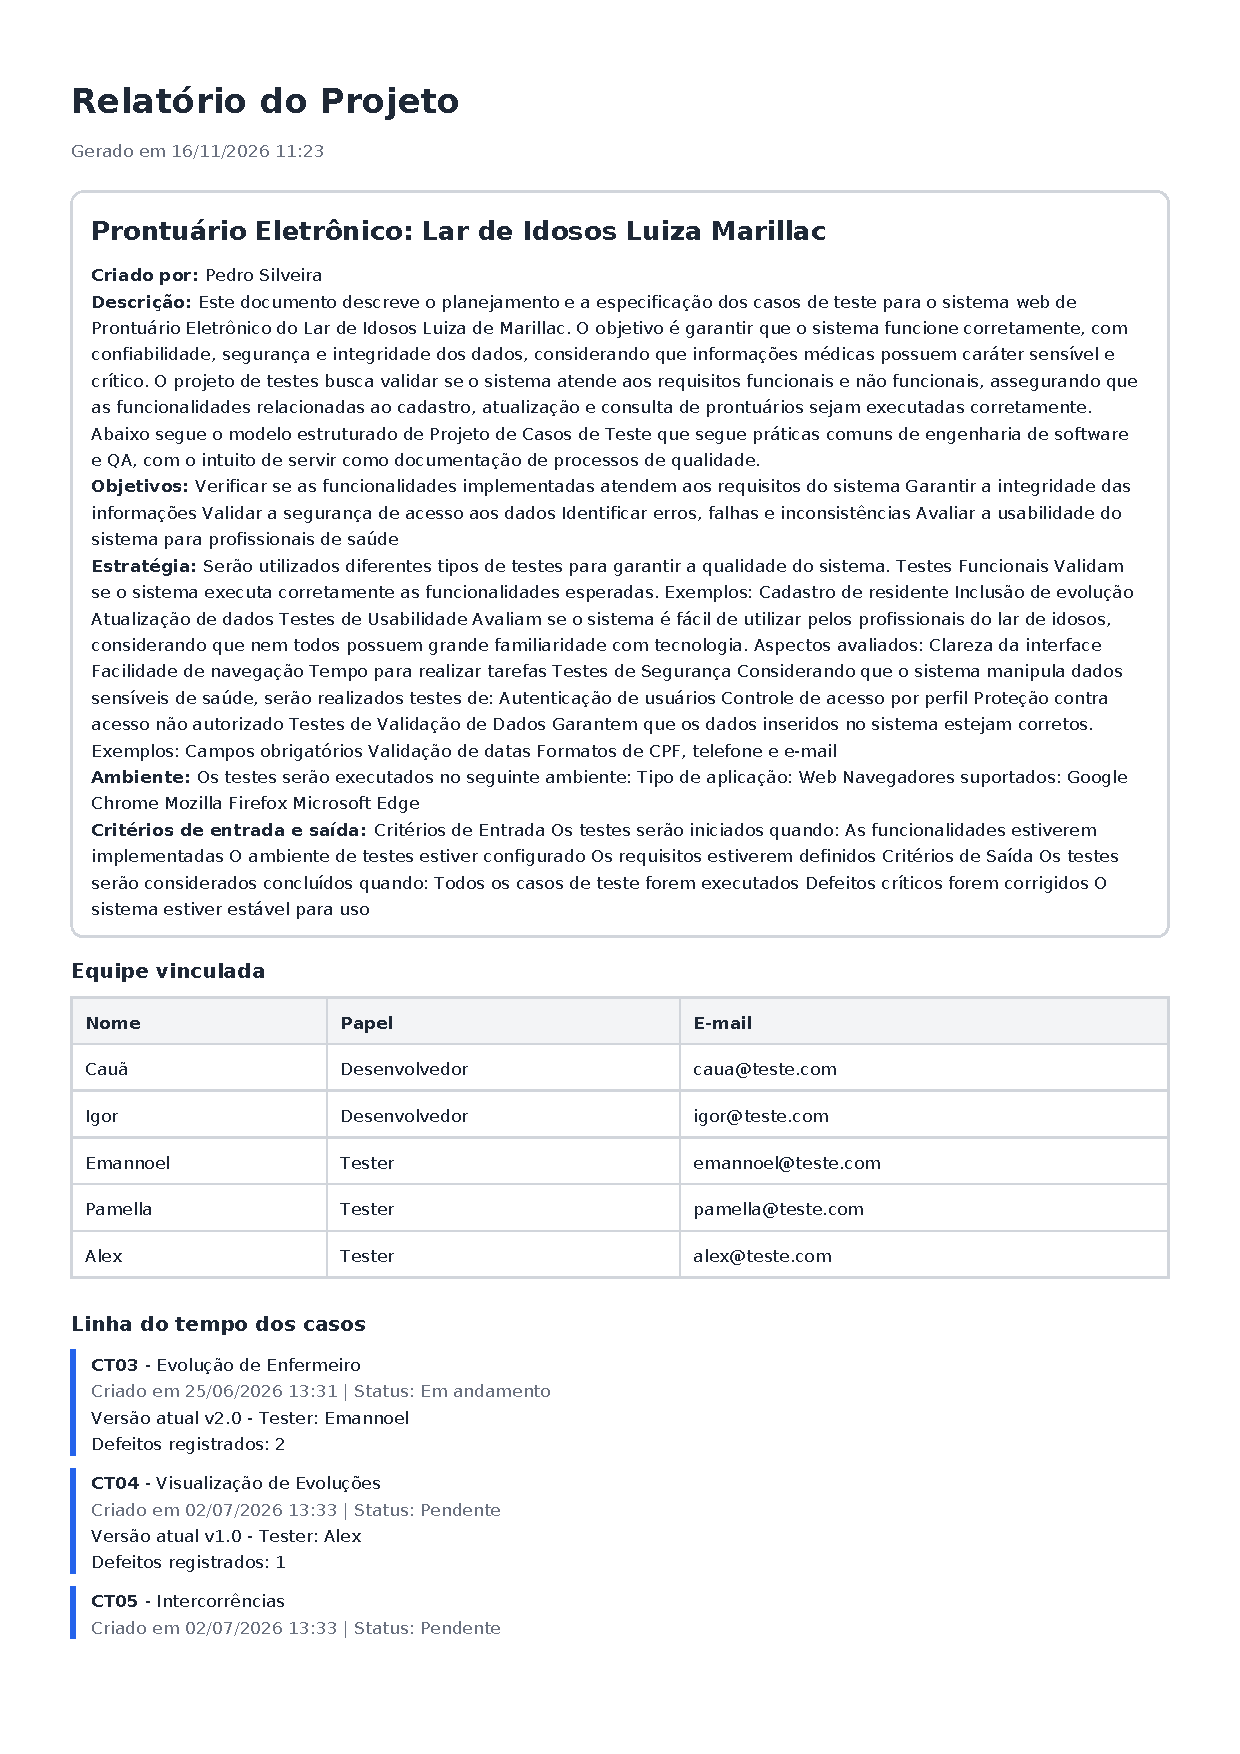
\includepdf[pages=-, scale=0.88, pagecommand={\thispagestyle{simple}}]{relatorio_projeto.pdf}
  \end{anexosenv}

  % Índice Remissivo
  \phantompart
  \printindex

\end{document}